%\documentclass[12pt,ascmac]{jreport}
\documentclass[12pt]{jreport}
\usepackage{./sty/eclepsf}
\usepackage{tascmac}
\usepackage{tabularx}
\usepackage[longnamesfirst]{natbib}
\usepackage[dvipdfmx]{graphics}
\usepackage[dvipdfmx]{graphicx}
\usepackage[dvipdfmx]{color}
\usepackage{subfigure}
\usepackage{alltt}
\usepackage{./sty/ncodeline}
%\usepackage[dvipdfmx, colorlinks, breaklinks,%
\usepackage[dvipdfmx, breaklinks,%
bookmarks=true, bookmarksnumbered=true,%
bookmarkstype=toc, bookmarksopen=true,bookmarksopenlevel=3,%
pdftitle={Proposal and Implementation of Latency Efficient Overlay Network (LEON)},%
%%pdfsubject={},%
pdfauthor={Yudai Yamagishi},%
pdfkeywords={1.Latency, 2.Distributed, 3.Overlay Network, 4.Layer 2 Network Extension}%
]{hyperref}
\usepackage{bookmark}

\AtBeginDvi{\special{pdf:tounicode EUC-UCS2}}

\usepackage{fancyhdr}

\usepackage{./sty/doxygenorig}

\usepackage{indentfirst}
\usepackage{url}
\usepackage{listings,./sty/jlisting}

\lstset{%
 language={C++},
 %backgroundcolor={\color[gray]{.85}},%
 basicstyle={\small},%
 identifierstyle={\small},%
 commentstyle={\small\itshape},%
 keywordstyle={\small\bfseries},%
 ndkeywordstyle={\small},%
 stringstyle={\small\ttfamily},
 frame={tb},
 breaklines=true,
 columns=[l]{fullflexible},%
 numbers=left,%
 xrightmargin=0zw,%
 xleftmargin=1.5zw,%
 numberstyle={\scriptsize},%
 stepnumber=1,
 numbersep=1zw,%
 lineskip=-0.5ex%
}

\usepackage{amssymb}
%\usepackage{supertabular,multirow}

% A4  size: 297mm*210mm %1pt = 0.35mm
\setlength{\topmargin}{-3.4mm} % 10pt 25.4mm - 3.4mm = 22mm
\setlength{\oddsidemargin}{-0.4mm} % 25.4mm - 0.4mm = 25mm
\setlength{\evensidemargin}{-0.4mm} % 25.4mm - 0.4mm = 25mm
\setlength{\textheight}{231mm} % 660pt % original is 225.75mm 645pt
\setlength{\textwidth}{160mm} % 457pt

\renewcommand{\topfraction}{.99}
\renewcommand{\textfraction}{.0}
\renewcommand{\floatpagefraction}{.99}
\renewcommand{\bibname}{参考文献}

\pagestyle{fancy}  
%\rhead{\thepage}
%\rhead[]{\leftmark} 
\lhead[]{} 
%\lhead[\rightmark]{} 

\makeatletter
\def\chaptermark#1{\markboth {\ifnum \c@secnumdepth>\m@ne
\@chapapp\ \thechapter \@chappos\ \fi #1}{}}
\makeatother

\begin{document}

\pagenumbering{roman}

\begin{titlepage}
  \begin{center}
    \begin{large}
      卒業論文   2015年度(平成27年)\\
      \vspace{24pt}
      Self-host化によるSwiftコンパイラのソースコード可読性の向上
      \end{large}
  \end{center}
  \vspace{40em}
  \begin{flushright}
    \large 慶應義塾大学 環境情報学部\\
    出水 厚輝
  \end{flushright}
\end{titlepage}


\thispagestyle{empty}
卒業論文要旨 - 2015年度 (平成27年度)
\begin{center}
\begin{Large}
\begin{tabular}{|c|} \hline
Self-host化によるSwiftコンパイラのソースコード可読性の向上
\\ \hline
\end{tabular}
\end{Large}
\end{center}
%~ \bigskip ~ \\

オープンソースとなったソフトウェアにおいては、その開発に関わるプログラマの増加とそれに伴うプログラムの修正や機能追加の増加によって、そのソースコードの可読性が拡張やそれに対するレビューの容易さに影響し、プロジェクト自体の成否に大きく関わる場合がある。

2015年12月にオープンソースとなったApple社が中心となって開発しているプログラミング言語Swiftもそうした可能性の分岐点に立つソフトウェアの1つである。
現在Swiftコンパイラの可読性は既存コードのコーディングスタイルへの習慣的な追従とレビューの徹底によって保たれているが、この形だけでは新しいコードの増加やプロジェクトメンバーの交代などによってその可読性が保てなくなる可能性が高い。

一方で、Swiftでは行われていないものの、現在利用されている多くの高級な汎用プログラミング言語では、コンパイル対象となる言語自体でそのコンパイラを記述するSelf-host化がよく行われている。
Self-host化を行うことによるメリットはいくつかあるが、たびたびモチベーションとしてあげられるのは、その可読性における優位点である。
コンパイラを記述する言語とその対象言語が同じになれば開発者はより少ない知識でコンパイラのコードを読むことができる上、初期のコンパイラにおいては、それを記述している言語よりもそのコンパイル対象となっている言語のほうが必ず後発のものであるため、多くの場合により表現力が高く、可読性においてもより高い水準となるからである。

そこで本研究では、Swiftで記述されたSwiftコンパイラの構文解析器を実装し、現行のSwiftコンパイラの構文解析器とそのソースコードの行数を多面的に比較することでSelf-host化がSwiftコンパイラに与える影響についての検証を行った。
検証の結果として、本論文ではSwiftコンパイラのSelf-host化によってその可読性が向上する可能性が十分にあることを示している。
だだし、同時に行ったSelf-host化に伴うデメリットの考察により、Self-host化がコンパイラに対して与える他の影響を鑑みると、実際の適用に際してはより慎重にならなければいけないということもわかった。

~ \\
キーワード:\\
\underline{1. コンパイラ},
\underline{2. Self-host化},
\underline{3. プログラムの可読性},\\
\underline{4. プログラミング言語Swift}
\begin{flushright}
慶應義塾大学 環境情報学部\\
出水 厚輝
\end{flushright}

\clearpage

\thispagestyle{empty}
Abstract of Bachelor's Thesis - Academic Year 2015
\begin{center}
\begin{large}
\begin{tabular}{|p{0.97\linewidth}|}
    \hline
    Improvement of the Readability of Swift Compiler's Source Code by Self-hosting\\
    \hline
\end{tabular}
\end{large}
\end{center}

~ \\

When the software project changes into an open source, as both the number of joining developpers \& the extension/modification of program increase, the readability of software's source code becomes important factor for succeeding the project.

In December 2015, the Swift programming language project, which is leaded by Apple, made its souce code public and started to face with such a change.
In current process, the readability of Swift compiler is maintained just by the effort to habitually follow the coding style of existing codes and its strict review.
Therefore, when the new codes grows wider in the software, its readability should become out of control.

On the other hand, there is a technique called Self-hosting, which is adopted in many general-purpose high-level programming languages.
The Self-hosting is a technique writing the compiler in its targeting programming language.
Although there are multiple reasons to adopt the Self-hosting to the compile, the most attractive advantage is that developers can reduce their effort for understanding the software.
When the compiler is self-hosted, its developpers are not reqired to learn the other than the targeting language.
And furthermore, as the targeting language is newer than its compiler's description language in the early years, the Self-hosting has an effect to change the compiler's source code less complex with the new and expressive grammars of targeting language.

In this research, we implemented the new Swift compiler which is written by Swift and compare its parser with the parser of Apple's Swift compiler in order to verify the readability enhancement ability of Self-hosting.
As the result of this research, we colud confirm the positive effect of Self-hosting on the readability.
But at the same time, as the effect depends on some characteristic grammars of Swift, we are considering that some other languages whose compiler is written by other high-level language may not be benefited the effect.

~ \\
Keywords : \\
\underline{1. Compiler},
\underline{2. Self-hosting},
\underline{3. Readability of Program},\\
\underline{4. Swift Programming Language}
\begin{flushright}
Keio University, Faculty of Environment and Information Studies\\
Atsuki Demizu
\end{flushright}

\clearpage

\tableofcontents\thispagestyle{empty} %目次
\clearpage
\listoffigures\thispagestyle{empty} %図目次
\clearpage
\listoftables\thispagestyle{empty} %表目次
\clearpage
\pagenumbering{arabic}
\chapter{序論}
\label{introduction}

\section{背景}
\label{introduction:background}

2015年12月4日、Apple社が予てより同社の提供するCocoaおよびCocoa Touchフレームワークを用いたソフトウェアの開発用として提供していたプログラミング言語Swiftをオープンソース化し、Linuxを中心としたさまざまなプラットフォームにおけるソフトウェアを開発するための拡張を開始した。
これによりプログラミング言語SwiftはObjective-Cの担ってきたiOSやMac OS Xなどにおけるソフトウェアの開発だけでなく、C++やJavaなど他の汎用プログラミング言語が担ってきたソフトウェア開発においても、それらの代替となり得る可能性を持つこととなった。

Swiftはオブジェクト指向や全称型・存在型の導入、関数の第一級オブジェクト化、HindlyとMilnerによる型再構築アルゴリズムの採用など、現在多くのプログラマに使用されている他の汎用高級言語が持つ様々な特徴を持っているが、まだその特徴を採用するか否かがよく議論されていないものもある。
その内の1つがコンパイラをそのコンパイル対象の言語自体で開発するBootstrapプロセスの採用である。

表~\ref{table:bootstrapping-languages}はWeb検索エンジンにおけるクエリヒット数からプログラミング言語の知名度を格付けしたTIOBE Indexの2015年12月版において上げられている言語の内、汎用言語であるものだけを上位から20言語抽出し、それらの主要なコンパイラがその言語自体で記述されているかを示したものである。
この20言語の内だけでもBootstrapを行っているものが8言語あり、 その中に性能の問題からコンパイラ用の言語として採用されづらいインタプリタ型言語なども含まれていることを考慮すれば、かなりの言語がBootstrapされていることが分かる。
しかし、現在SwiftはC++を用いて開発されており、Bootstrapは行われていない。

現在Swiftにおいては未だ多くの機能が不足しており、他の問題を優先しているためにBootstrapについて大きく取り上げられてはいない。
また、開発者のメーリングリスト~\cite{dev-ml}では特にSwiftコンパイラのバックエンドとして採用されているLLVMのAPIがC++で提供されていることから、SwiftがC++と同様の役割を果たすにはもう少し時間が必要だという意見も上がっている。


しかし、~\ref{explain-bootstrap:merit}節で述べるようにBootstrapを行うことで得られる利益があることが他の言語の事例によって示されている以上、十分な議論なしに現状のSwiftにBootstrapが不要であると判断するのは早計であるといえる。

\begin{table}[tb]
    \begin{center}
        \caption{知名度の高いプログラミング言語のBootstrap状況}
        \begin{tabular}{|c|c|c|c|}
            \hline
            順位 & 言語名 & コンパイラ名 & Bootstrap状況 \\
            \hline
            1 & Java & javac & N (C, C++?) \\
            \hline
            1 & Java & OpenJDK & N (C++, Java) \\
            \hline
            2 & C & gcc & N (C++) \\
            \hline
            2 & C & clang & N (C++) \\
            \hline
            3 & C++ & gcc & Y \\
            \hline
            3 & C++ & clang & Y \\
            \hline
            3 & C++ & Microsoft Visual C++ & Y \\
            \hline
            4 & Python & cpython & N (C) \\
            \hline
            4 & Python & PyPy & Y \\
            \hline
            5 & C\# & Microsoft Visual C\# & N (C++) \\
            \hline
            5 & C\# & .NET Compiler Platform (Roslyn) & Y \\
            \hline
            6 & PHP & Zend Engine & N (C) \\
            \hline
            7 & Visual Basic .NET & Visual Studio & N (C++, C\#) \\
            \hline
            7 & Visual Basic .NET & .NET Compiler Platform (Roslyn) & Y \\
            \hline
            8 & JavaScript & SpiderMonkey & N (C, C++) \\
            \hline
            8 & JavaScript & V8 & N (C++, JavaScript) \\
            \hline
            9 & Perl & perl & N (C) \\
            \hline
            10 & Ruby & Ruby MRI & N (C) \\
            \hline
            12 & Visual Basic & Visual Studio & N (C++, C\#) \\
            \hline
            13 & Delphi/Object Pascal & Delphi & N (?) \\
            \hline
            13 & Delphi/Object Pascal & Free Pascal & Y \\
            \hline
            14 & Swift & swift & N (C++) \\
            \hline
            15 & Objective-C & clang & N (C++) \\
            \hline
            15 & Objective-C & gcc & N (C++) \\
            \hline
            17 & Pascal & Free Pascal & Y \\
            \hline
            17 & Pascal & GNU Pascal & N (C, Pascal) \\
            \hline
            20 & COBOL & GnuCOBOL & N (C, C++) \\
            \hline
            21 & Ada & GNAT & Y \\
            \hline
            22 & Fortran & GNU Fortran & N (C, C++) \\
            \hline
            22 & Fortran & Absoft Fortran Compiler & ? \\
            \hline
            23 & D & DMD & Y \\
            \hline
            24 & Groovy & groovy & N (Java, Groovy) \\
            \hline
        \end{tabular}
        \label{table:bootstrapping-languages}
    \end{center}
\end{table}

% \begin{figure}
%     \begin{center}
%         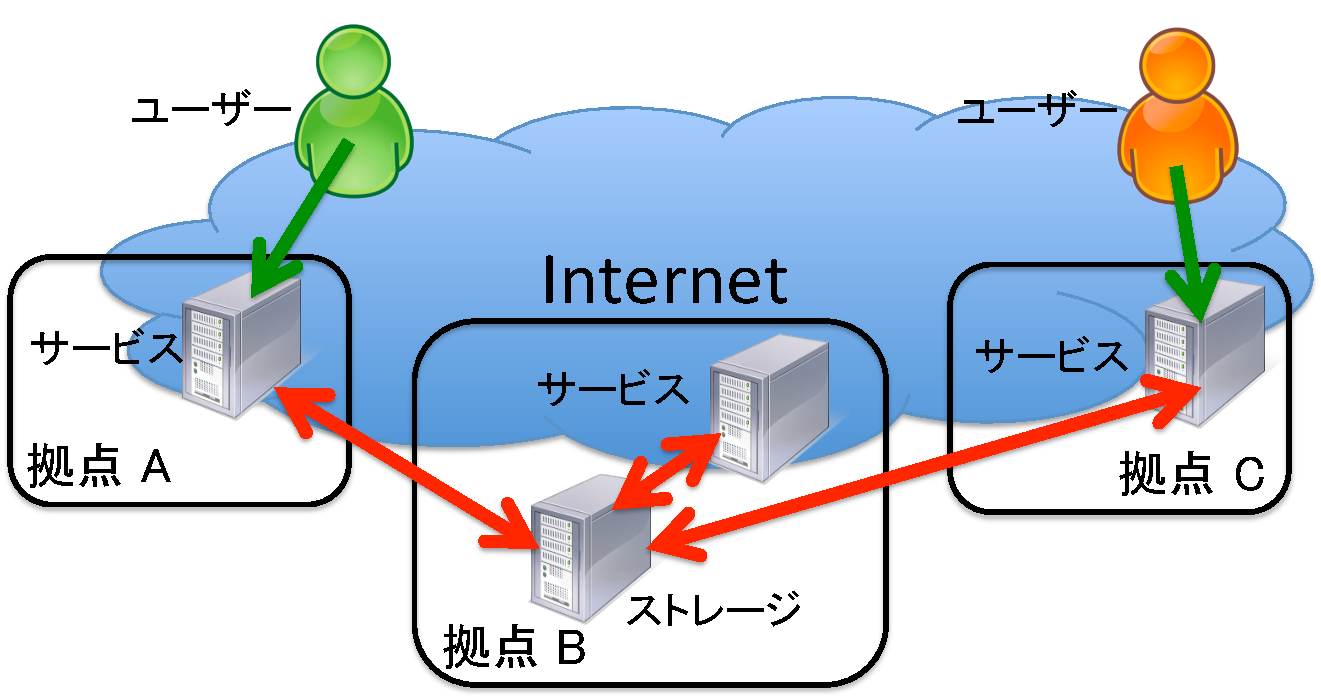
\includegraphics[scale=0.50]{./img/serviceanduser}
%         \caption{複数の拠点から提供されるサービス}
%         \label{img:mlservice}
%     \end{center}
% \end{figure}


\section{本研究が着目する課題}
\label{introduction:issue}

Swiftコンパイラが抱える他の問題との優先度や使用しているフレームワークとのつなぎ込みに関する問題が解決したとしても、SwiftコンパイラのBootstrapを行うかどうかという判断を下すにはより根源的な課題がある。
それは、現在Swiftを記述しているC++言語がSwiftと比較しても高い表現力を持っているために、~\ref{explain-bootstrap:instance}節で見る幾つかの事例とは異なり、Bootstrapを行うことで得られるメリットや、そもそも現行のコンパイラで使用されている手法を維持したままBootstrapを行うことが可能であるか否かが自明でないというものである。

また、現在のSwiftはC++との相互運用性を持っていないため、コンパイラ中の一部分をSwiftで記述したものに置き換えることは難しく、逆に実際に使用されているコンパイラ中のモジュール化が可能なほど大きなパーツをSwiftへ移植するとなると、その間の言語への機能追加などの改変は現行のものと移植中のものの両者に適用するか、移植中のもののみに追加して移植が完了するまでその適用を先送りしなくてはならなくなってしまう。


\section{本研究の目的}
\label{introduction:purpose}

本研究では、SwiftコンパイラがBootstrapすることによって得られるメリットと被るデメリットを定量的に示し、Bootstrapを行うべきか否かを判断する上で有用な情報を収集することを目的とする。
そのためのアプローチとして、Swiftコンパイラの基幹的機能である構文解析器をSwiftによって実装し、その実行時間とソースコードの行数を現行のSwiftコンパイラの構文解析器と比較する。
また、この独自の構文解析器は現行のSwiftコンパイラと基本的な設計手法において同じものを採用するだけで、完全に独立させたものとして実装する。

この方法により、現在のSwiftコンパイラの開発状況などの影響を一切受けずにBootstrapのための評価が可能となり、またその評価がBootstrapの可能性に対して有意義な知見を与えることを提示する。


\section{本論文の構成}

本論文の構成は次の通りである。

第2章では本研究の考察対象であるコンパイラのBootstrapについてSwift以外の言語の事例からそのメリットについてまとめ、Bootstrapにおける課題について整理する。
第3章では本研究が着目するプログラミング言語Swiftの特徴とそのコンパイラ実装の基幹部分における特徴について説明する。
第4章では現行のSwiftコンパイラとの比較対象となるSwiftで記述したSwiftコンパイラ「TreeSwift」の構成について述べ、現行のコンパイラとその基本的な設計手法などに大きな差異がないことを確認する。
第5章では現行のSwiftコンパイラとTreeSwiftの構文解析器についてその実行速度とソースコードの行数を比較し、その結果について考察する。
第6章では本研究の結論と今後の展望についてまとめる。

%%% Local Variables:
%%% mode: japanese-latex
%%% TeX-master: "../thesis"
%%% End:

\chapter{関連研究}
\label{rw}

\begin{figure}[h]
	\begin{center}
		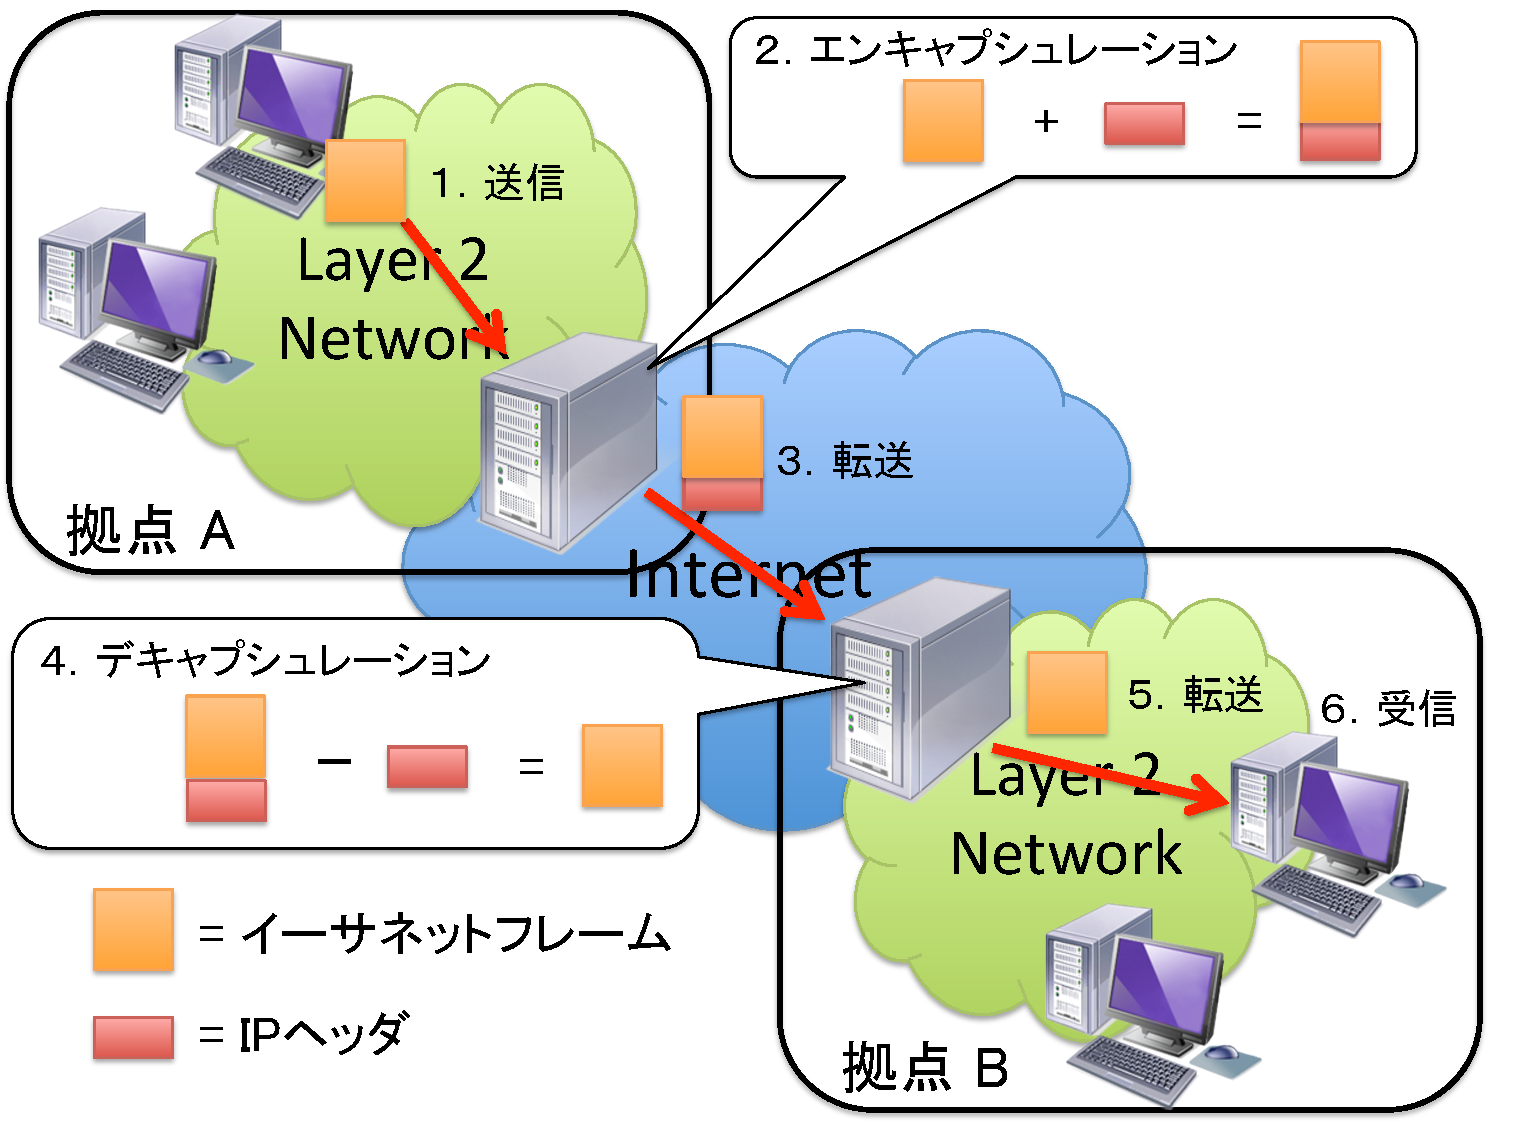
\includegraphics[scale=0.50]{./img/l2tunnel}
		\caption{Layer 2ネットワークの拡張手法}
		\label{img:l2tunnel}
	\end{center}
\end{figure}

Layer 2ネットワーク拡張技術を利用することにより、インターネット上に分散された複数の拠点に同一の
Layer 2ネットワークを拡張することができる。広域に分散した複数の拠点でサービスを展開するためには、
サービスを構成しているコンポーネントを拠点間で共有する必要がある場合が多い。広域に分散した複数の拠点間で
、共通のセキュリティーポリシーが適用された状態で、共通のコンポーネントを利用する手法の1つとしてLayer 2ネットワーク
拡張技術を利用するという手法が挙げられる。Layer 2ネットワーク拡張技術はインターネット上でLayer 2ネットワーク
のイーサネットフレームを転送することにより、仮想的に広域なLayer 2ネットワークを構築する。

Layer 2ネットワーク拡張技術はトンネル終端点となるコンピューターがスイッチのように動作する。動作の仕組みを図~\ref{img:l2tunnel}に示す。まず、Layer 2ネットワーク
拡張技術を利用して構築されたLayer 2ネットワーク上のホストが、トンネルの反対側にいるコンピューター宛のイーサネットフレーム
を送信する。それを受信したトンネル終端点は、受信したイーサネットフレームの先頭に、宛先が反対側のトンネル終端点となっている
IPヘッダーを追加(=エンキャプシュレーション)して送信する。そして、エンキャプシュレーション
されたイーサネットフレームを受信したトンネル終端点は、追加されたIPヘッダーを取り除く(=デキャプシュレーション)。
最後に、宛先のホストへイーサネットフレームを転送する。これによりLayer 2ネットワークを拡張している。

既存のLayer 2ネットワーク拡張技術は、一対一型のLayer 2トンネル技術と一対多型のLayer 2トンネル技
術の2種類に分類することができる。以下で、それぞれの詳細を述べる。

\section{一対一型のLayer 2ネットワーク拡張技術}
\label{rw:pointtopoint}

\begin{figure}
	\begin{center}
		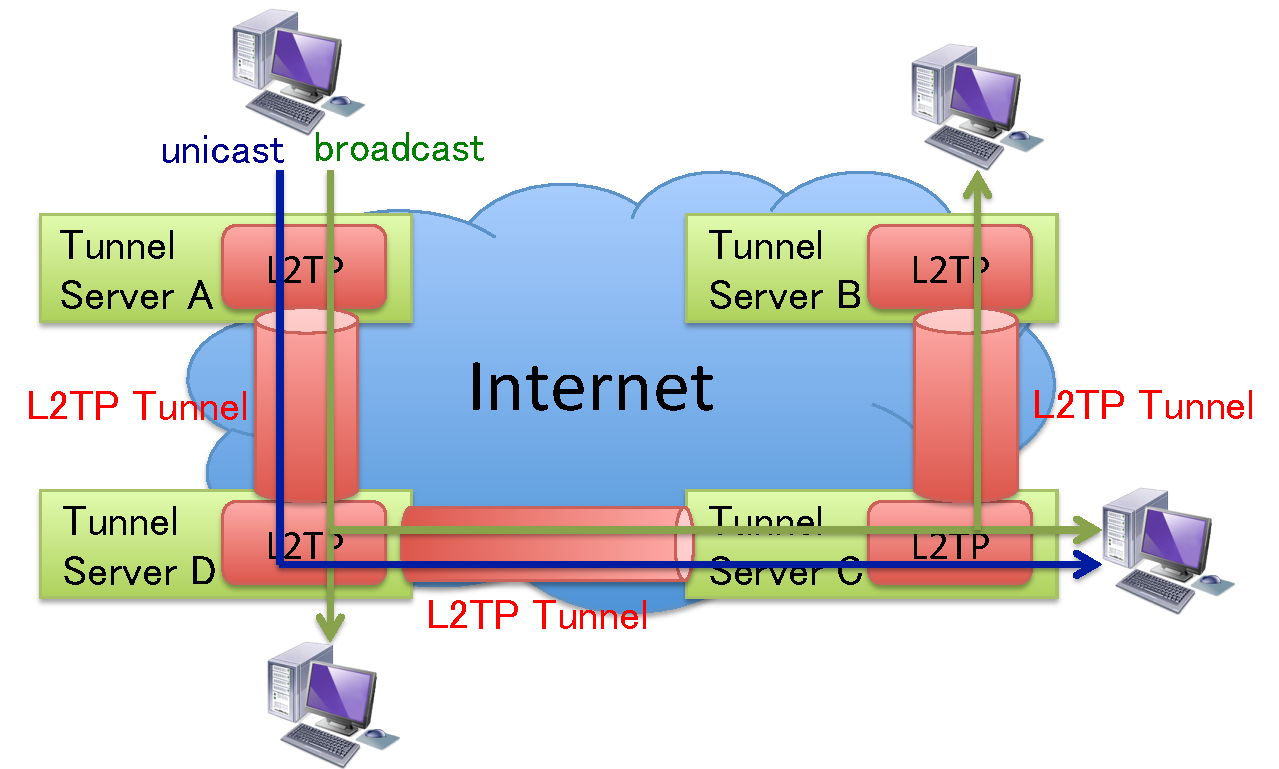
\includegraphics[scale=0.60]{./img/l2tptopology}
		\caption{L2TPを利用して拡張されたLayer 2ネットワーク}
		\label{img:l2tptopology}
	\end{center}
\end{figure}

一対一型のLayer 2ネットワーク技術は2つの拠点間で拡張されたLayer 2ネットワークを構築することができる。
一対一型のLayer 2ネットワーク拡張技術の例として、L2TP~\cite{rfc:l2tp}やGRE~\cite{rfc:gre}トンネルなどが挙げられる。L2TPを利用して
Layer 2ネットワークを拡張した際のトポロジーを図~\ref{img:l2tptopology}に示す。一対一型の
Layer 2ネットワーク拡張技術では2拠点間でLayer 2ネットワークを拡張する。3拠点以上
に同一のLayer 2ネットワークを拡張するためには、一対一型のLayer 2ネットワーク拡張技術を動作さえ、
全ての拠点に同一のLayer 2ネットワークを拡張する。そのため、図~\ref{img:l2tptopology}で示したような
トポロジーとなる。しかし、この手法では一部の拠点間で行われる通信の遅延が大きくなってしまうという問題がある。

Layer 2ネットワークのトポロジーは必ず木構造のトポロジーとなる。Layer 2スイッチはブロードキャスト
やマルチキャストのイーサネットフレームを受信すると、そのイーサネットフレームを受信したポート以外の全ポートにイーサネットフレーム
を転送する(=フラッディング)。フラッディングされたイーサネットフレームを受信したLayer 2スイッチは同様ににその
イーサネットフレームをフラッディングする。そのため、リング型のトポロジーでは、ブロードキャストストームや
マルチキャストストームが発生してしまうという問題(=L2ループ)が生じる。L2ループが生じると帯域がブロードキャストやマルチキャストの
イーサネットフレームで専有されてしまう上に、Layer 2スイッチのCPU負荷が高くなり正常にイーサネットフレームを
転送できなくなる。その結果、Layer 2スイッチに接続されているホスト同士も通信不能となってしまう。このような問題
を防ぐために、Layer 2ネットワークは木構造のトポロジーで構築される。また、Spanning Tree Protocol(=STP)を利用することで、
L2ループを発生させずにリング型のトポロジーを構築することも可能だが、
STPはL2ループを防ぐためにリングとなっているポートの通信を拒否する。その結果、STPを利用した場合でも、Layer 2ネットワークの
トポロジーは木構造のトポロジーとなってしまう。

\begin{figure}
	\begin{center}
		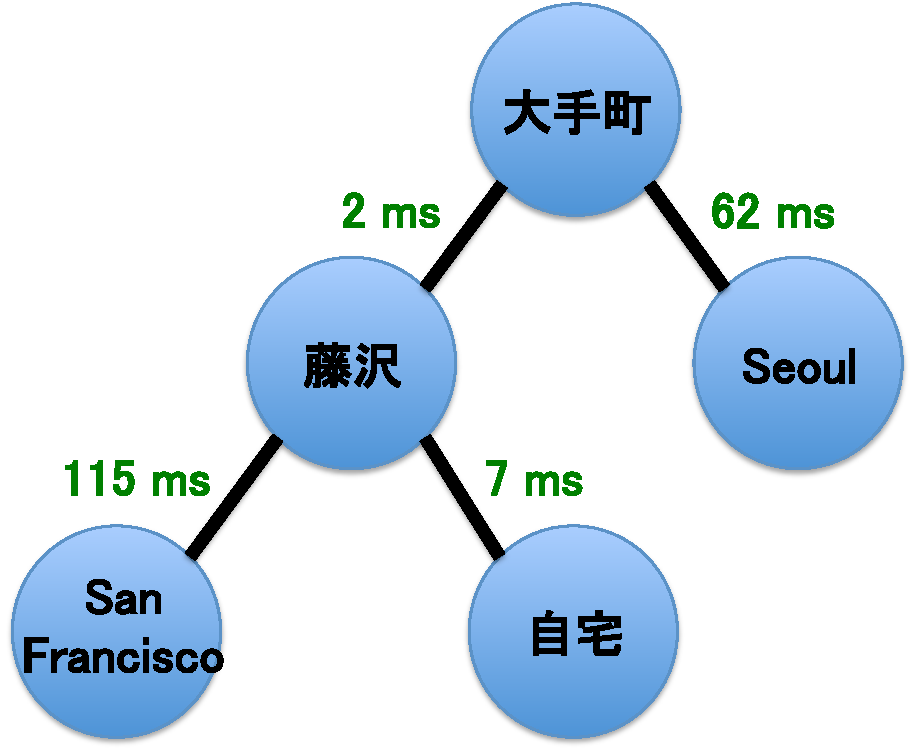
\includegraphics[scale=0.50]{./img/highlatencyl2}
		\caption{木構造となる広域Layer 2ネットワークのトポロジー例1}
		\label{img:highlatencyl2}
	\end{center}
\end{figure}

\begin{figure}
	\begin{center}
		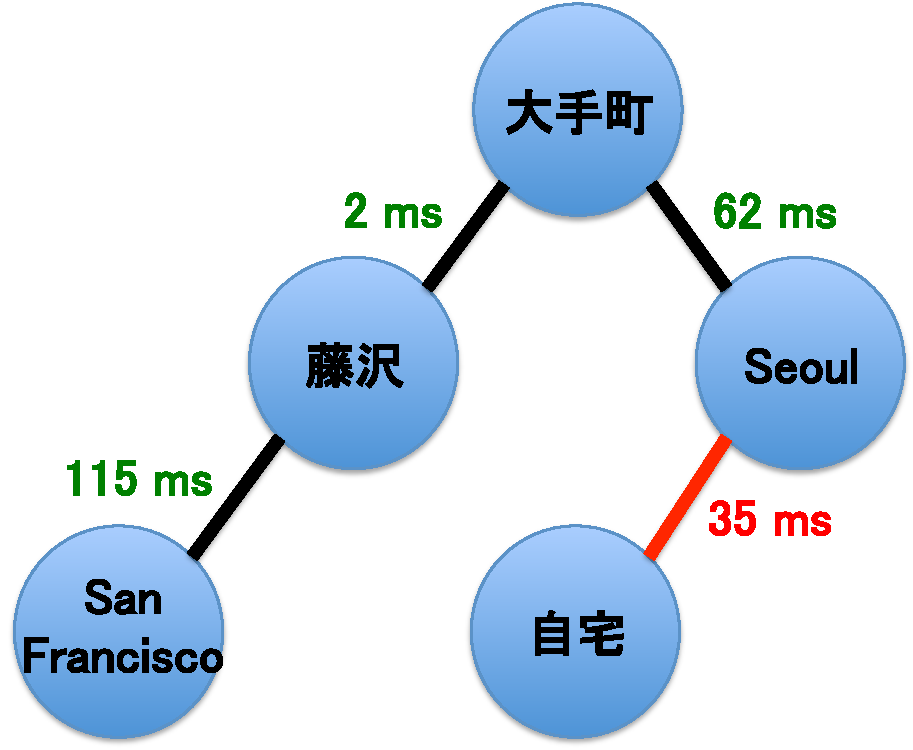
\includegraphics[scale=0.50]{./img/homeandseoul}
		\caption{木構造となる広域Layer 2ネットワークのトポロジー例2}
		\label{img:homeandseoul}
	\end{center}
\end{figure}

一対一型のLayer 2ネットワーク拡張技術を利用し、Layer 2ネットワークを複数の拠点に拡張した場合も
同様に木構造のトポロジーとなる。単一の拠点内で構築されるLayer 2ネットワークの場合、
Layer 2スイッチ間の遅延はほぼ無い状態なので、木構造のトポロジーでも問題とならない。しかし、Layer 2ネットワーク拡張技術を利用して
インターネット上に構築したLayer 2ネットワークでは、1ホップあたりの遅延が、単一の拠点内で構築したLayer 2ネットワークと比べ、非常に大きい。例えば、図~\ref{img:highlatencyl2}
で示すような広域なLayer 2ネットワークでは、自宅に設置されたホストとソウルに設置されたホスト間で通信を行った
場合、その遅延は71 msとなる。図~\ref{img:homeandseoul}で示すように、自宅とソウルを直接
接続した場合、遅延は35 msとなる。しかし、藤沢や大手町に設置されたホスト間で通信を行った
場合の遅延が97 ms以上となってしまう。このように、一対一型のLayer 2ネットワーク拡張技術では、
Layer 2ネットワークのトポロジーが木構造となってしまうため、必ず一部拠点間の遅延が大きくなってしまうという問題がある。


\section{一対多型のLayer 2ネットワーク拡張技術}
\label{rw:pointtomulti}

\begin{figure}
	\begin{center}
		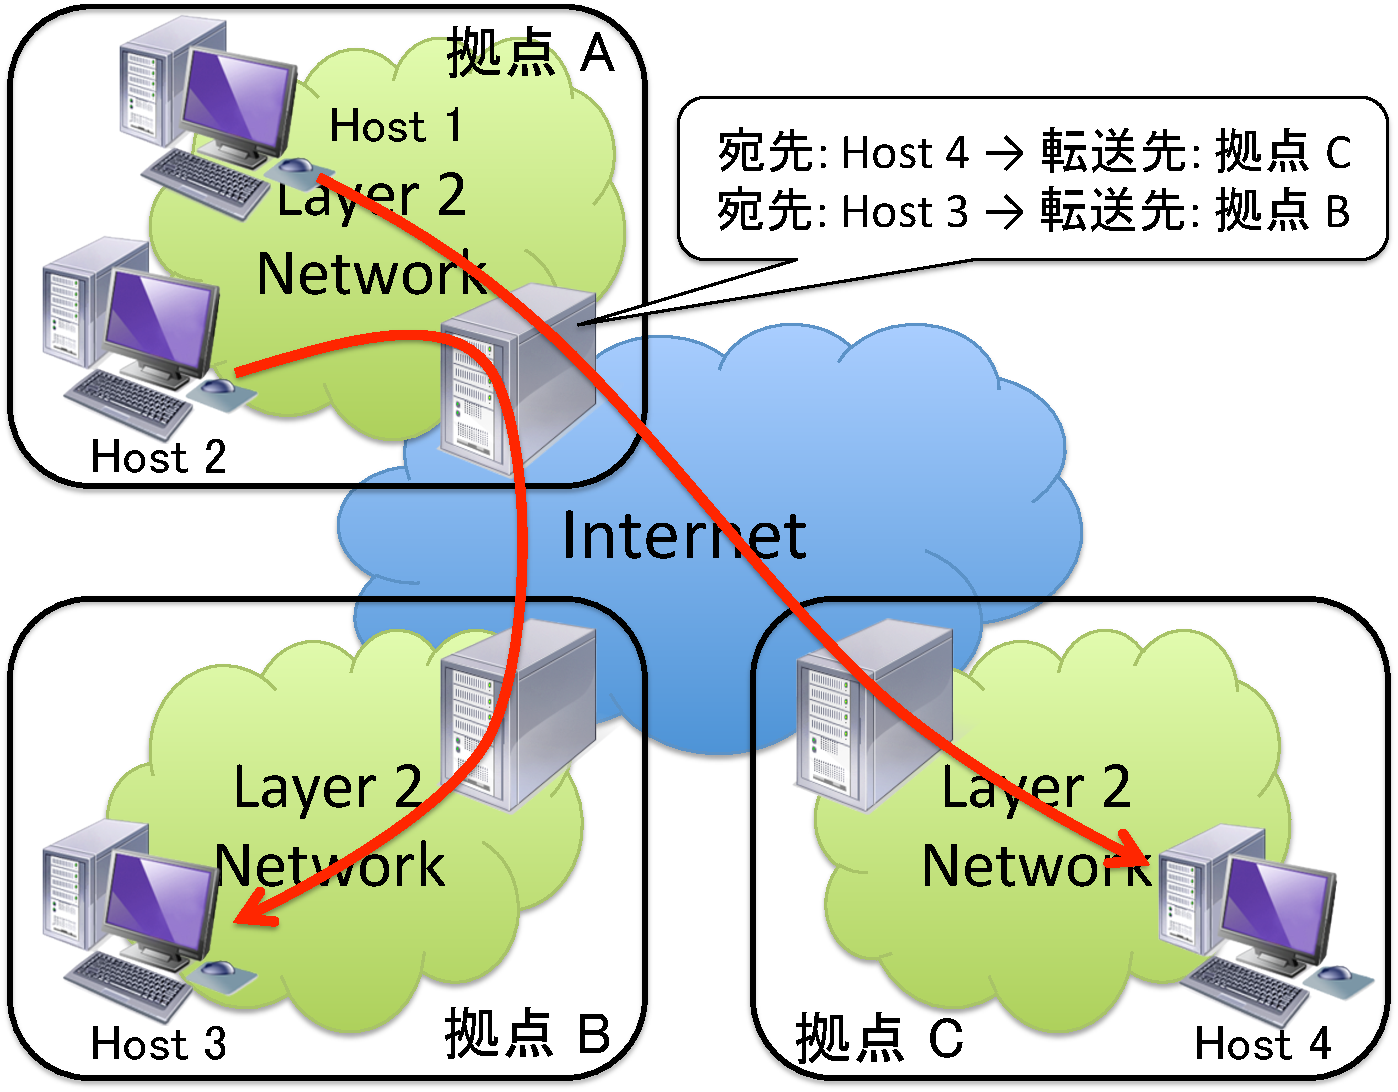
\includegraphics[scale=0.50]{./img/1tomulti}
		\caption{一対多型のLayer 2ネットワーク拡張技術}
		\label{img:1tomulti}
	\end{center}
\end{figure}

一対多型のLayer 2ネットワーク拡張技術は複数の拠点に対して同時にLayer 2ネットワークを拡張
することができる。一対一型のLayer 2ネットワーク拡張技術では、構築されたLayer 2ネットワーク
が木構造のトポロジーとなってしまうため、必ず一部拠点間の遅延が大きくなってしまうという問題がある。
この問題は、Layer 2ネットワーク拡張技術が、図~\ref{img:1tomulti}で示すように、
イーサネットフレームの宛先ホストに応じて転送するトンネル終端点の切り替えを行うことにより解決することが
できる。Layer 2ネットワーク拡張技術は、各拠点に設置されているホストを自動的に学習する。そして、
イーサネットフレームを転送する際には、宛先ホストがどのトンネル終端点によって収容されているか検索し、
そのトンネル終端点にイーサネットフレームを直接転送する。この手法では、一対一型のLayer 2ネットワーク拡張技術と比べると、
イーサネットフレームが宛先のトンネル終端点に直接
転送されるため、遅延の小さいLayer 2ネットワークを構築することができる。

一対多型のLayer 2ネットワーク拡張技術の例としてVirtual Extensible Local Area Network(=VXLAN)~\cite{id:vxlan}
とN2N~\cite{n2n}が挙げられる。これらの特徴を以下で述べる。

\subsection{VXLAN}
\label{rw:vxlan}

\begin{figure}
	\begin{center}
		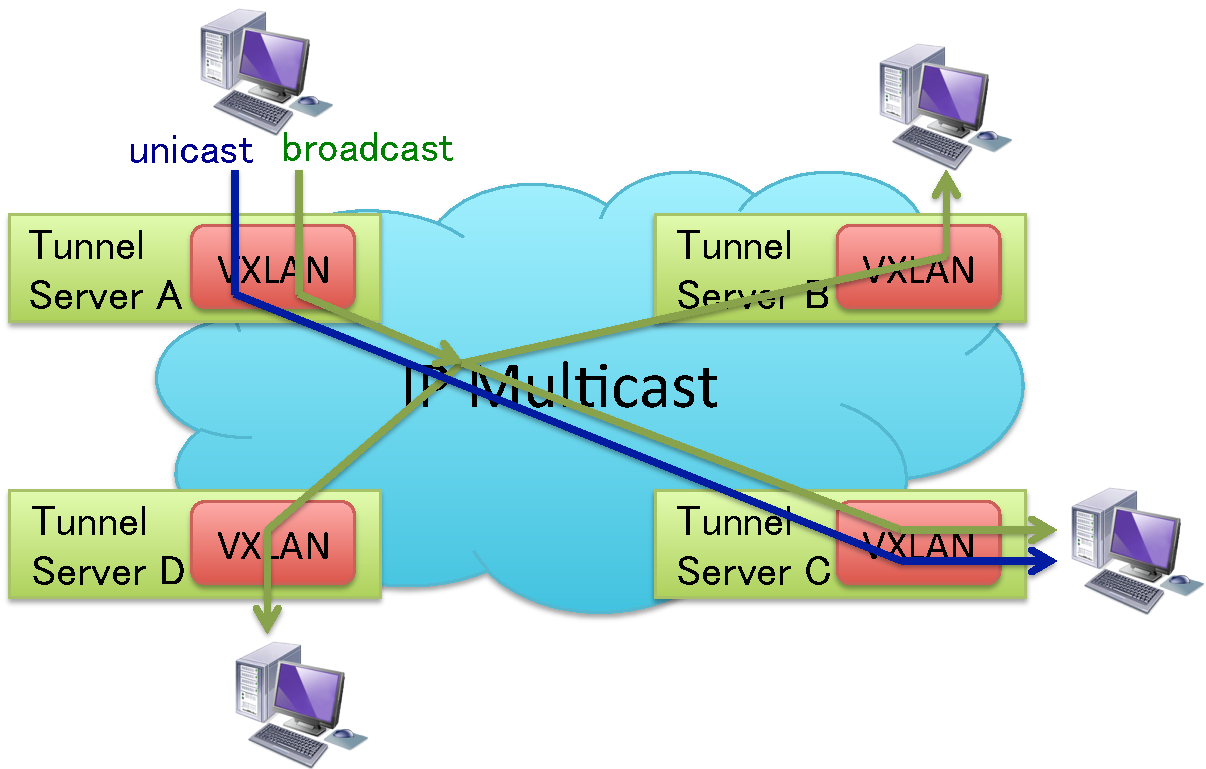
\includegraphics[scale=0.60]{./img/vxlantopology}
		\caption{VXLANを利用して拡張されたLayer 2ネットワーク}
		\label{img:vxlantopology}
	\end{center}
\end{figure}

VXLAN~\cite{id:vxlan}はCisco Systems社~\cite{cisco}やVMware社~\cite{vmware}を中心に提案されている一対多型のLayer 2ネットワーク拡張技術である。
VXLANを利用することにより、同一のLayer 2ネットワークを複数の拠点に拡張することができる。
VXLANを利用して複数の拠点に同一のLayer 2ネットワークを拡張した際のトポロジーとVXLANの
イーサネットフレーム転送手法を図~\ref{img:vxlantopology}に示す。
VXLANはトンネル終端点の検知やブロードキャストフレームの転送を行うために、IPマルチキャスト
を利用する。拡張されたLayer 2ネットワークに参加しているトンネル終端点は、全て同一の
IPマルチキャストグループに参加している。トンネル終端点が、収容しているホストからイーサネットフレームを
受信すると、まずそのイーサネットフレームの識別を行う。受信したイーサネットフレームが、ブロードキャストフレームの場合、
IPマルチキャストを利用してイーサネットフレームを転送する。全てのトンネル終端点は同一のIPマルチキャスト
グルームに参加しているため、IPマルチキャストグループに受信したイーサネットフレームを転送することにより、
イーサネットフレームは全てのトンネル終端点へ転送される。そして、他のトンネル終端点がそのイーサネットフレームを受信すると、
イーサネットフレームを収容しているホストへ転送する。また、イーサネットフレームを受信したトンネル終端点はイーサネットフレームの送信元ホストと
イーサネットフレームを転送したトンネル終端点を学習する。受信したイーサネットフレームがユニキャストフレームの場合、
まず、イーサネットフレームの宛先ホストが学習されているか確認する。学習されている場合、
受信されたイーサネットフレームを宛先ホストが収容されているトンネル終端点に直接転送する。学習されていない場合、
ブロードキャストフレームと同様に、IPマルチキャストを利用し全てのトンネル終端点へイーサネットフレームを転送する。
そして、宛先ホストが収容されているトンネル終端点がイーサネットフレームを受信すると、そのイーサネットフレーム
を宛先ホストへ転送する。VXLANは上記手法により、同時に複数の拠点に同一のLayer 2ネットワークを
拡張する。

VXLANを利用することにより、一対一型のLayer 2ネットワーク拡張技術で生じる木構造トポロジーの問題は解決
される。VXLANは転送されてきたイーサネットフレームの送信元ホストと転送したトンネル終端点を自動的に学習する。
そして、学習された情報を元に、転送すべきイーサネットフレームの宛先ホストに応じて転送先を自動的に選択する。
転送すべきイーサネットフレームがブロードキャストフレームの場合、または、学習されていないホスト宛のユニキャスト
フレームの場合はIPマルチキャストグループに転送する。学習されているホスト宛のユニキャストフレームの
場合は、宛先ホストが収容されているトンネル終端点に直接転送する。これにより、一対一型のLayer 2ネットワーク
拡張技術で生じる不要な中継がなくなるため、遅延は一対一型のLayer 2ネットワーク拡張技術と比べると小さくなる。

しかし、VXLANはインターネット上で動くように設計されていないため、VXLANを利用してインターネット上
に分散した複数の拠点に同一のLayer 2ネットワークを拡張するのは困難である。VXLANはトンネル終端点の
検知と一部イーサネットフレームの転送にIPマルチキャストを用いる。そのため、全てのトンネル終端点は同一の
IPマルチキャストグループに参加していることが求められる。しかし、インターネット上に分散した複数の
拠点に同一のIPマルチキャストグループを拡張することは困難である。XCast~\cite{rfc:xcast}やScatterCast~\cite{scattercast}などといった
IPマルチキャストを利用して、インターネット上に分散した複数の拠点に同一のIPマルチキャストグループを
拡張することは可能だが、Layer 2ネットワークを拡張をするために動かさなければいけないシステムが増える
ため、運用コストが高くなる上に障害発生時の問題切り分けも難しくなる。そのため、VXLANはインターネット上
の複数の拠点に同一のLayer 2ネットワークを拡張する手法として適切ではない。

また、VXLANを利用してインターネット上の複数の拠点に同一のLayer 2ネットワークを拡張した場合、
イーサネットフレームは遅延が最も小さい経路で転送されない。インターネット上の経路には~\ref{background:internetroute}節
で説明したように、直接転送した場合より、他のトンネル終端点を経由したほうが遅延が小さくなる場合がある。
VXLANはこのような経路が存在した場合でも、それを検知する仕組みが存在しないため、イーサネットフレームの転送は
必ず宛先のトンネル終端点に直接行う。そのため、拡張されたLayer 2ネットワークの遅延は最小限とならない。

\subsection{N2N}
\label{rw:n2n}

\begin{figure}
	\begin{center}
		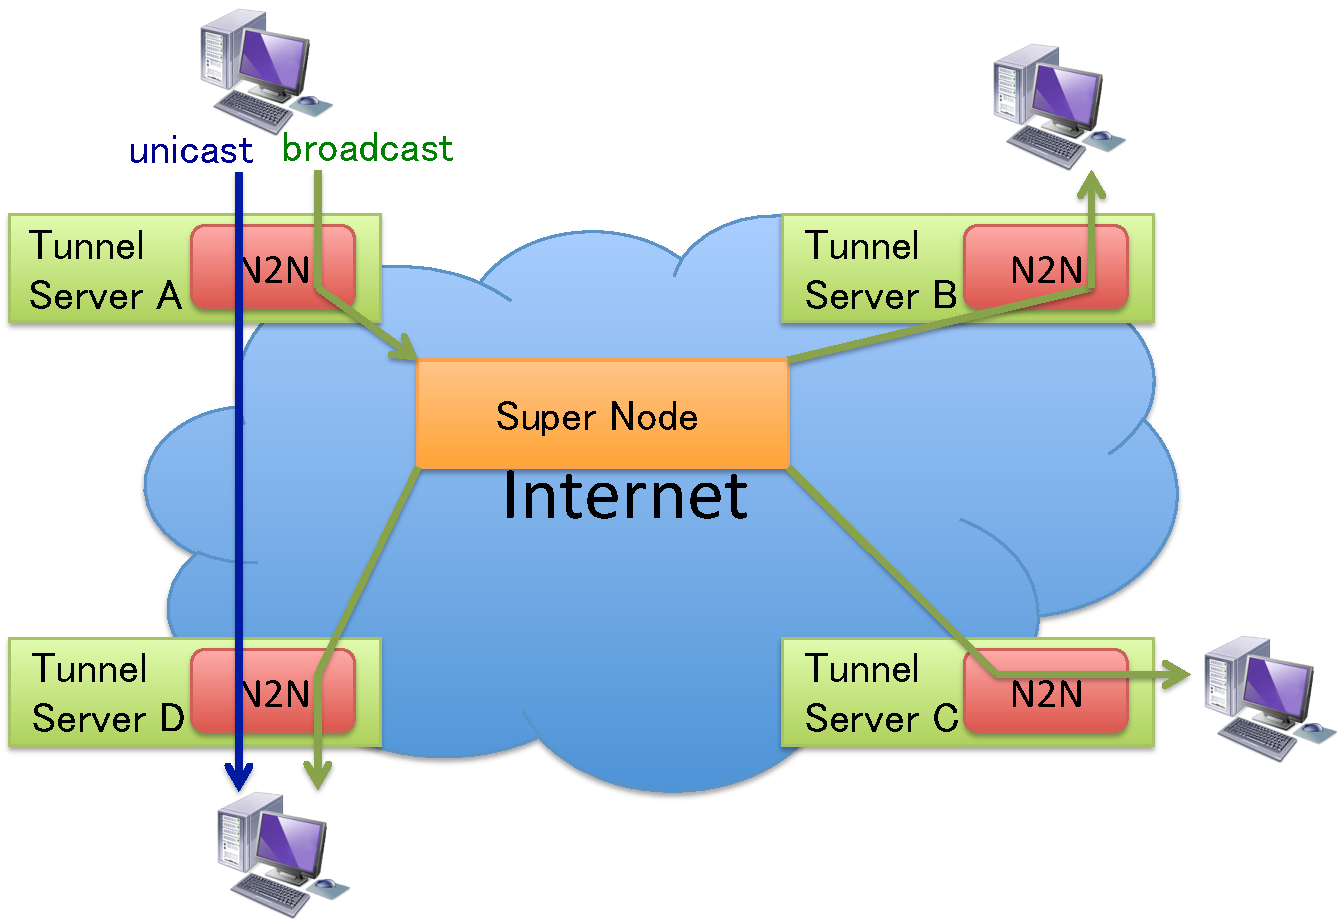
\includegraphics[scale=0.60]{./img/n2ntopology}
		\caption{N2Nを利用して拡張されたLayer 2ネットワーク}
		\label{img:n2ntopology}
	\end{center}
\end{figure}

N2N~\cite{n2n}はntop社~\cite{ntop}によって開発されている一対多型のLayer 2ネットワーク拡張技術である。
N2Nを利用することにより、インターネット上に分散した複数の拠点に同一のLayer 2
ネットワークを拡張することができる。N2Nを利用してインターネット上に分散した
複数の拠点に同一のLayer 2ネットワークを拡張した際のトポロジーとN2Nの
フレーム転送手法を図~\ref{img:n2ntopology}に示す。

N2Nはインターネット上に分散した複数の拠点に同一のLayer 2ネットワークを拡張する
ために、トンネル終端点とは別に、Supernodeというサーバーを用いる。Supernodeの役割
は大きく分けて2つある。1つ目の役割は、トンネル終端点の参加や離脱などといったコントロールメッセージ
の通知と管理である。Supernodeはトンネル終端点がLayer 2ネットワークへ参加した際に、Layer 2ネットワークに参加
している全トンネル終端点にそれを通知する。新規トンネル終端点はSupernodeのIPアドレスとポート番号を指定するだけで、Layer 2ネットワークに参加することができる。
2つ目の役割は、ブロードキャストフレームと一部ユニキャストフレームの転送である。
トンネル終端点がブロードキャストフレームを転送するためには、Supernodeにブロードキャストフレーム
を転送し、Layer 2ネットワークに参加している全トンネル終端点にブロードキャストフレームを転送してもらう。
これによりN2Nはインターネット上に分散した複数の拠点に同一のLayer 2ネットワークを
拡張することを可能としている。

N2Nはイーサネットフレームを宛先のトンネル終端点に直接転送するため、一対一型のLayer 2ネットワーク
拡張技術のように、一部通信の遅延が大きくなってしまうという問題が生じない。
N2Nによって拡張されたLayer 2ネットワークに参加しているホストがイーサネットフレームを
送信すると、N2Nのトンネル終端点はそのイーサネットフレームの転送を行う。トンネル終端点が
受信したイーサネットフレームがブロードキャストフレームの場合、トンネル終端点はそのイーサネットフレーム
をSupernodeに転送する。そして、Supernodeは受信したイーサネットフレームを全てのトンネル終端点
に転送する。Supernodeが再転送を行ったブロードキャストフレームをトンネル終端点が受け取ると、
収容しているホストにイーサネットフレームを転送した上で、送信元ホストと転送をしたトンネル終端点を学習する。
トンネル終端点が受信したイーサネットフレーム
がユニキャストフレームの場合、ユニキャストフレームの宛先ホストが学習されているホストかを確認する。
学習されているホストの場合は宛先ホストが収容されているトンネル終端点にイーサネットフレームを直接
転送する。学習されていないホストの場合はブロードキャストフレームと同様に、Supernodeへ転送し、全
トンネル終端点に転送を行なってもらう。N2Nはこのようにイーサネットフレームを宛先のトンネル終端点
に直接転送をするため、遅延は一対一型のLayer 2ネットワーク拡張技術と比べ小さくなる。

しかし、N2Nは~\ref{background:internetroute}節で説明したようなインターネットの経路が考慮されていない。
また、一部のイーサネットフレームは必ずSupernodeを経由する。そのため、遅延が最も小さい経路で転送されていないと言える。N2Nにはトンネル終端点間の
遅延を計測し、その計測結果に基いて遅延が最も小さい経路を選択する仕組みが存在しない。そのため、
他のトンネル終端点を経由することにより遅延が小さくなるような経路が存在したとしても、イーサネットフレーム
は宛先のトンネル終端点に直接転送される。また、ブロードキャストフレームや一部のユニキャストフレームは必ず
Supernodeを経由する。そのため、トンネル終端点からSupernodeまでの遅延が大きい場合や、Supernodeの負荷が高い
場合は遅延が大きくなってしまう。よって、N2Nではインターネット上に分散した複数の拠点に拡張されたLayer 2ネットワーク
の遅延は最小限とならない。

更にN2NはSupernodeが単一障害点となっている。N2Nは一部イーサネットフレームの転送にSupernodeを用いている。
また、Layer 2ネットワークに参加しているトンネル終端点の管理はSupernodeが行なっている。そのため、
Supernodeで障害が発生した場合、拡張されたLayer 2ネットワークが完全に利用できなくなってしまうという問題がある。

\section{関連研究の比較}
\label{background:korekara}

本節では、~\ref{rw:pointtopoint}節、~\ref{rw:pointtomulti}節で説明したLayer 2ネットワーク拡張技術について、
インターネット上に分散された複数の拠点に同一のLayer 2ネットワークを拡張した際に、拡張されたLayer 2ネットワーク上で
動作するサービスの遅延によるパフォーマンス低下を小さくするという目的に向けた観点から比較、検討を行う。これを実現するための
要件は以下の通りである。

\begin{itemize}
	\item{宛先に応じた転送先の選択が可能である}
	\item{遅延が最も小さくなる経路の選択が可能である}
	\item{インターネット上で動作する}
	\item{分散して動作する}
\end{itemize}

目的を実現するための各要件について、~\ref{rw:pointtopoint}節と~\ref{rw:pointtomulti}節で挙げた既存研究が
どの程度満たしているかを表~\ref{table:relatedworks}に示す。

\begin{table}[h]
	\begin{center}
		\caption{既存研究の比較}
		\begin{tabular}{|c|c|c|c|c|}
			\hline
			既存研究 & 転送先の選択 & 遅延に基づいた経路選択 & インターネットでの動作 & 分散 \\
			\hline
			\hline
			L2TP,GRE & × & × & ◯ & × \\
			VXLAN & ◯ & × & × & ◯ \\
			N2N & ◯ & × & ◯ & × \\
			\hline
		\end{tabular}
		\label{table:relatedworks}
	\end{center}
\end{table}

~\ref{background:thisresearch}節で説明したように、インターネット上に分散された複数の拠点に拡張した
Layer 2ネットワークで動作するサービスの遅延によるパフォーマンス低下を小さくするためには、イーサネット
フレームを遅延が最も小さくなる経路で転送する。L2TPやGREといった一対一型のLayer 2ネットワーク拡張技術
は、転送先をイーサネットフレームの宛先に応じて選択することができない。そのため、Layer 2ネットワークの
トポロジーは木構造となるため、一部通信の遅延は大きくなる。一方、N2NとVXLANは宛先に応じて転送先を選択
することができる。しかし、N2NとVXLANには、トンネル終端点間の遅延を計測し、その計測結果に基いて遅延が
最も小さくなる経路を選択する仕組みがない。そのため、転送する際の経路が、必ずしも遅延の最も小さい経路
ではないという問題がある。

また、インターネット上に分散された複数の拠点に同一のLayer 2ネットワークを拡張するためには、Layer 2ネットワーク
拡張技術がインターネット上で動作する必要がある。L2TP、GREとN2Nはインターネット上で動作するように設計されている。
しかし、VXLANは他トンネル終端点の検知と一部イーサネットフレームの転送にIPマルチキャストを用いているため、
インターネット上では動作しないという問題がある。

更に、~\ref{background:ml2}項で説明したように、1つの拠点で発生した障害によるサービスの停止を防ぐために、
複数の拠点を利用する場合が多い。拡張されたLayer 2ネットワークが、ある拠点で発生した障害の影響を受け、
利用できなくなっては複数拠点の利点を得ることが出来ない。VXLANは分散して動作しているため、IPマルチキャストが
正常に動作していれば、障害の影響は受けない。一方で、L2TPとGREは木構造のトポロジーとなるため、ある拠点で
障害が発生すると拡張されたLayer 2ネットワークでも障害が発生する、という問題がある。また、N2NはSupernodeを利用してSupernodeの
管理と一部イーサネットフレームの転送を行なっているため、Supernodeが設置されている拠点で障害が発生すると、
Layer 2ネットワークで一切通信ができなくなる、という問題がある。

%\begin{figure}
%	\begin{center}
%		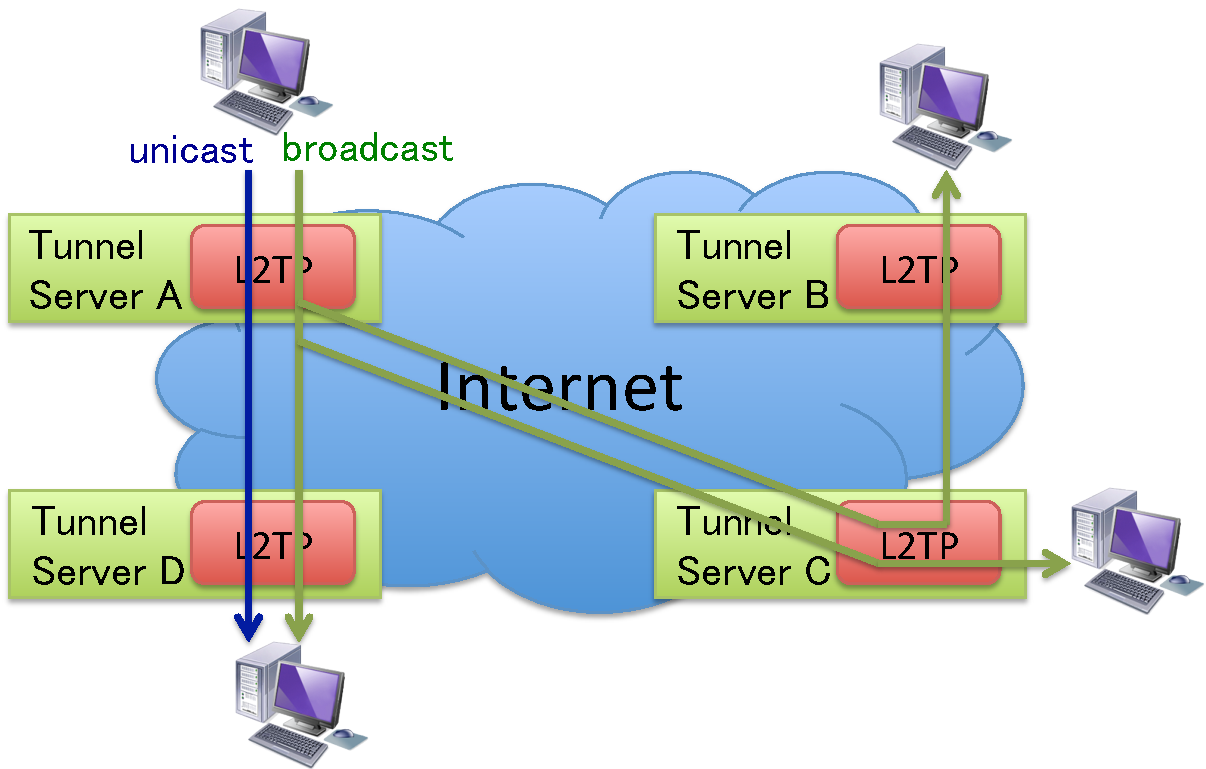
\includegraphics[scale=0.60]{./img/leontopology}
%		\caption{求められるLayer 2ネットワーク拡張技術}
%		\label{img:reqtopology}
%	\end{center}
%\end{figure}

%%% Local Variables:
%%% mode: japanese-latex
%%% TeX-master: "../yummy_bthesis"
%%% End:

\chapter{提案手法}
\label{solv}

本章では、低遅延な広域Layer 2ネットワークを構築するにあたり想定する環境を整理した上で、本研究で
提案するシステムの概要について述べる。

\section{設計}

\begin{figure}
	\begin{center}
		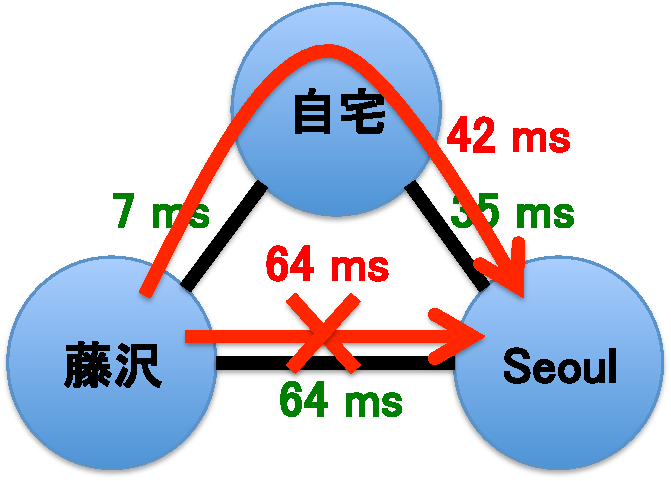
\includegraphics[scale=0.60]{./img/betterpath}
		\caption{他拠点を経由させることによる遅延の削減}
		\label{img:betterpath}
	\end{center}
\end{figure}

本研究では、まずトンネル終端点が、トンネル終端点間の遅延を計測し、その計測結果に基づいた経路選択が行えるようにする。
例えば、図~\ref{img:betterpath}で示すように、藤沢、自宅とソウルの3拠点に同一のLayer 2ネットワークを拡張するとする。この場合、
藤沢とソウルの間で通信するにあたり、インターネットの経路で直接転送するよりも、自宅を経由
することにより約35\%小さい遅延で通信することが可能である。Layer 2ネットワーク拡張技術は、このような経路を発見するために、
Layer 2ネットワークに参加している全トンネル終端点の遅延を計測する。そして、遅延が最も小さくなる経路を計測結果から計算し、その経路でイーサネットフレームの
転送を行う。

また、インターネット上で分散して動作するよう、トンネル終端点が個々でLayer 2ネットワークに参加しているトンネル終端点のリスト
を管理するようにする。トンネル終端点はLayer 2ネットワークへの参加や離脱などのメッセージを、Layer 2ネットワークに参加している
全てのトンネル終端点に広告する。これにより、全てのトンネル終端点でLayer 2ネットワークに参加しているトンネル終端点のリストを共有する。
また、全てのトンネル終端点に転送する必要があるイーサネットフレームは、SupernodeやIPマルチキャストに転送するのではなく、全てのトンネル終端点に1つ1つ転送する。
これにより、SupernodeやIPマルチキャストが不要となり、インターネット上で分散して動作するLayer 2ネットワークを構築することができる。


\section{想定環境}
\label{solv:env}

本研究の目的は、インターネット上でサービスを提供しているサービスプロバイダーが、
インターネット上に分散された複数の拠点に同一のLayer 2ネットワークを拡張する際に、拡張されたLayer 2ネットワーク上で
動作するサービスの遅延によるパフォーマンス低下を小さくすることである。
拠点の数は数十拠点を想定する。また、拠点の場所は国内、及び、その近隣諸国とする。インターネット上
に拠点が分散しているような環境では、現在のインターネットに存在する経路の問題に
より、宛先と直接通信するより、別の拠点を経由して宛先に到達するほうが
低遅延で通信できる場合がある。そこで本研究では、遅延を小さくするために、イーサネットフレームを転送する際に
遅延の最も小さい経路で転送をすることができるLayer 2ネットワーク拡張技術を提案する。これが実現することにより、従来の手法
と比べ、拡張されたLayer 2ネットワーク上で動作するアプリケーション
のパフォーマンスが向上されることが期待される。

本研究では拡張されたLayer 2ネットワーク上で利用されるアプリケーションとしてNFSv3を
想定する。複数の拠点に分散したサービスを構築するためには、同じデータを全拠点
からアクセスできることが必要となる場合がある。複数の拠点から共通のデータを利用する手段として
NFSv3を利用するという手法が挙げられる。しかし、NFSv3は遅延がとても小さい、単一の拠点内で運用され
るように設計されているため、遅延の大きい環境で利用した場合、パフォーマンスが著しく低下する。本研究では
このような低遅延を要求するアプリケーションを想定アプリケーションとする。

\section{機能要件}
\label{solv:requirements}

前節で説明したような環境で、低遅延な拡張されたLayer 2ネットワークを実現するための
Layer 2ネットワーク拡張技術に対する要件は以下の通りである。

\begin{itemize}
	\item{インターネット上に分散された複数の拠点へのLayer 2ネットワークの拡張}
	\item{宛先に応じた転送先の選択}
	\item{遅延の最も小さい経路でのイーサネットフレームの転送}
	\item{分散して動作すること}
\end{itemize}

低遅延な拡張されたLayer 2ネットワークを構築するためには、遅延の最も小さい経路でイーサネットフレームが転送
される必要がある。これを実現するために、まずLayer 2ネットワーク拡張技術は参加している全てのトンネル終端点間の
遅延を計測し、その計測結果を用いて遅延が最も小さい経路を計算する。そしてトンネル終端点が、
イーサネットフレームを転送する際には、イーサネットフレームの宛先に応じて転送するトンネル終端点を選択し、
計算した経路に基いて転送を行う。宛先の
トンネル終端点に直接転送する場合が最も遅延の小さい経路の場合には直接転送をする。他のトンネル終端点を経由して宛先
に転送したほうが小さい遅延で転送できる場合は、他のトンネル終端点を中継する。また、
インターネット上に分散された複数の拠点にLayer 2ネットワークを拡張することができる必要がある。
さらに、どこかの拠点で障害が発生した場合でも、正常にLayer 2ネットワークが動作していることが求められる。
そのため、Supernodeなどといった中心となるサーバーやIPマルチキャストが必要なく、分散して動作する必要がある。

\section{システム概要}
\label{solv:requiredl2}

\begin{figure}
	\begin{center}
		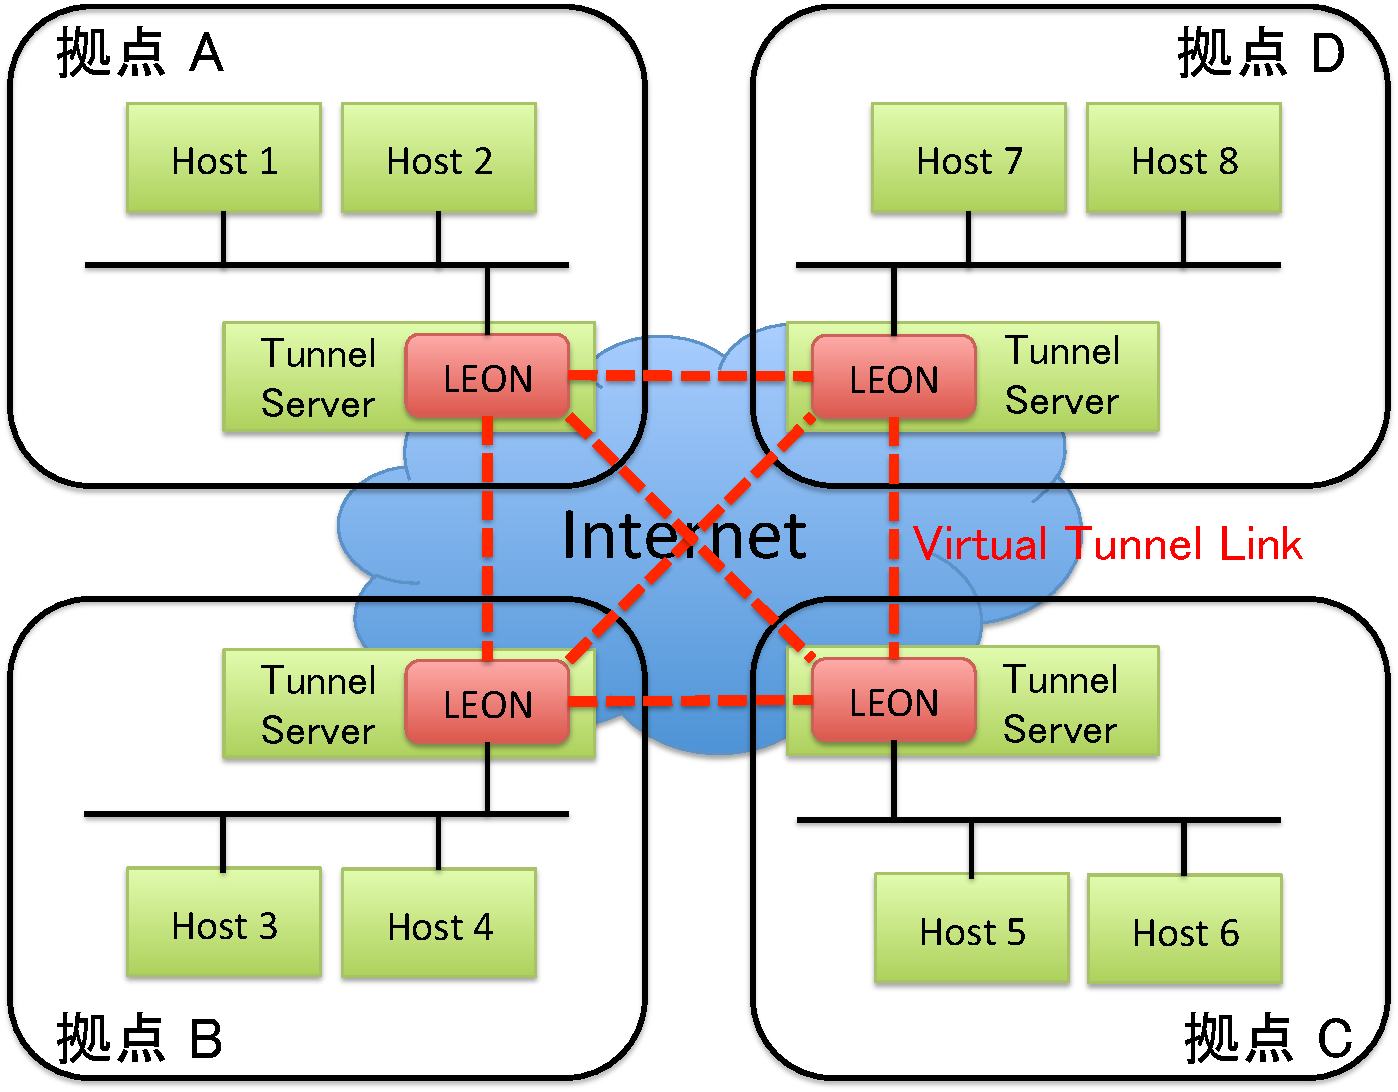
\includegraphics[scale=0.60]{./img/mtuntopology}
		\caption{LEONによって構築されるLayer 2ネットワークトポロジー}
		\label{img:mtuntopology}
	\end{center}
\end{figure}


本研究では、前節で示した機能要件を実現する低遅延Layer 2ネットワーク拡張手法として、
Latency Efficient Overlay Network (LEON)を提案する。LEONはIPネットワークを経由してイーサネットフレーム
を転送するLayer 2ネットワーク拡張技術である。LEONによって構築されるLayer 2ネットワーク
のトポロジーを図~\ref{img:mtuntopology}に示した。LEONを動かし、トンネル終端点として
動作するサーバーは各拠点に1つ設置する。トンネル終端点として動作するサーバーはインターネット
と拡張されたLayer 2ネットワークに所属するホストが収容されているLayer 2ネットワークに接続されている。
そして、LEONは自分の拠点に所属しているホストが、他拠点に設置されているホストと通信するための
ゲートウェイとして動作する。

\begin{figure}
	\begin{center}
		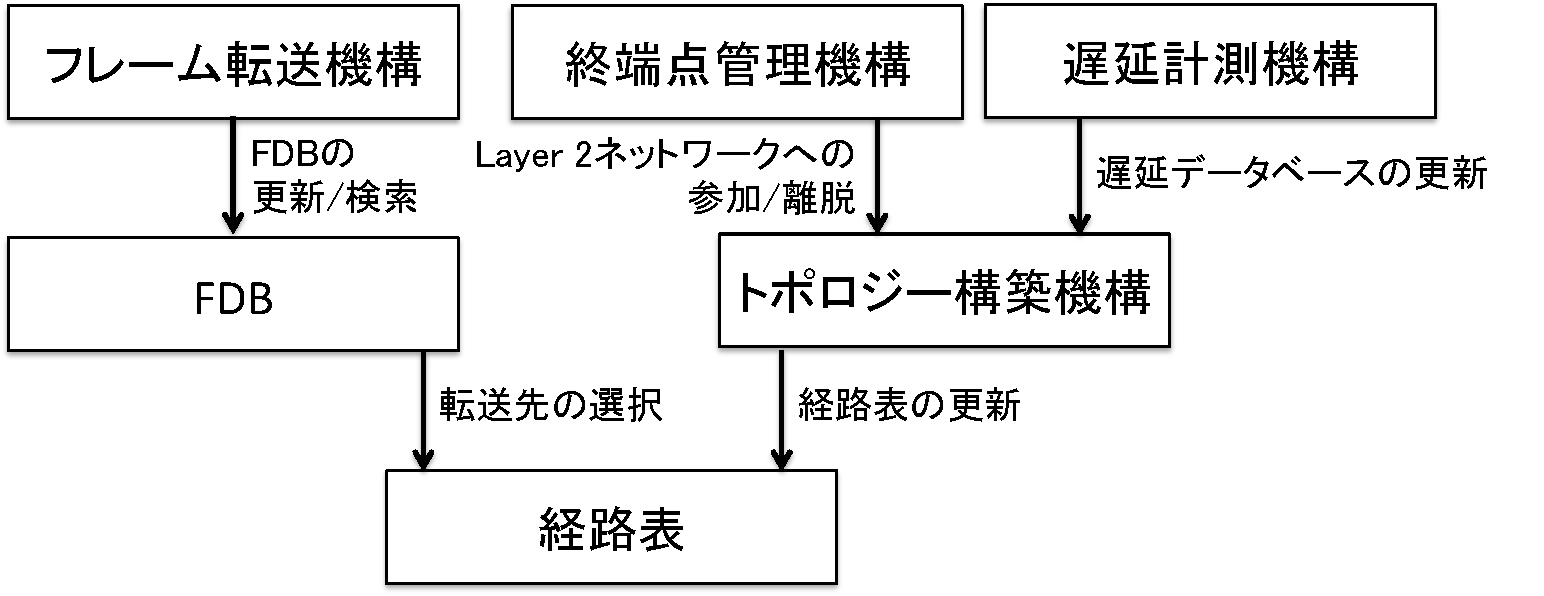
\includegraphics[scale=0.65]{./img/mtunworks}
		\caption{LEONのシステム概要}
		\label{img:mtuntopology}
	\end{center}
\end{figure}

LEONのシステム概要を図~\ref{img:mtuntopology}に示す。まず、LEONは既にLayer 2ネットワークに参加している
トンネル終端点を学習する。トンネル終端点の学習後、トンネル終端点間の遅延を計測する。トンネル終端点間の
遅延は時間帯に応じて変化する可能性があるため、トンネル終端点の学習時のみだけでなく、定期的に実行される。
また、遅延の計測結果は他トンネル終端点に広告する。そして、全てのトンネル終端点への遅延計測が完了後、
各トンネル終端点と通信する際に遅延が最も小さくなる経路を計算する。ここで計算された経路は経路表にする。
LEONが転送すべきイーサネットフレームを受信した際には、ホストがどのトンネル終端点に収容されているかが記録されている
データベースを参照し、イーサネットフレームの宛先ホストがどのトンネル終端点によって収容されているのか検索する。そして、
事前に計算された経路表に基づき、イーサネットフレームを宛先ホストが収容されているトンネル終端点へ転送する。

トンネル終端点の学習は、トンネル終端点を管理するサーバーなどを用いず、トンネル
終端点間で自律的に行う。トンネル終端点を管理するサーバーを用意することにより、Layer 2ネットワークに参加
しているトンネル終端点の学習やトンネル終端点間のメッセージングは容易となる。しかし、トンネル終端点を
管理するサーバーが単一障害点となってしまい、障害発生時には拡張されたLayer 2ネットワークの通信全体に
影響を与えてしまう可能性がある。トンネル終端点が自律的に他のトンネル終端点を学習できた場合、トンネル終端点
を管理するサーバーが必要なくなり、どれかのトンネル終端点で障害が発生したとしても、影響を受けるのは
障害が発生しているトンネル終端点だけである。そのため、LEONでは他トンネル終端点をトンネル終端点が
自律的に学習できるようにする。

\begin{figure}
	\begin{center}
		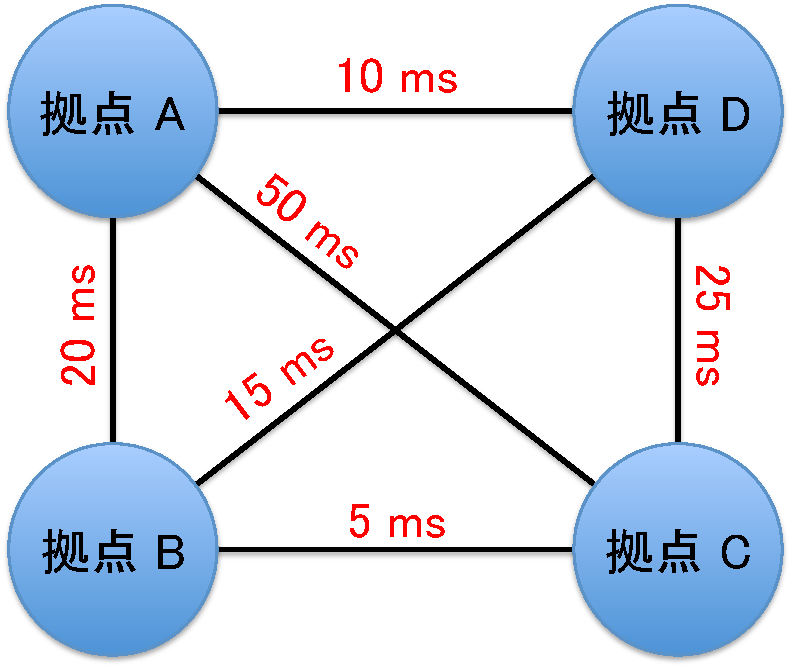
\includegraphics[scale=0.60]{./img/rttascost}
		\caption{RTTをコストとした経路の選択}
		\label{img:rttascost}
	\end{center}
\end{figure}

学習されたトンネル終端点へ到達するための経路は、トンネル終端点間の遅延に基いて選択する。
~\ref{background:internetroute}節で説明したように、現在のインターネット
の経路は宛先までの遅延やリンクの使用率などが考慮されていないため、遅延が最も小さい経路
でない場合がある。宛先にインターネットの経路で到達するよりも、他のトンネル終端点
を経由させたほうが遅延が小さくなる場合がある。そのため、遅延が最も小さい経路でイーサネットフレーム
を転送するためには、トンネル終端点は宛先のトンネル終端点に転送する際に、遅延が最も小さい経路
を計算する必要がある。LEONは、遅延が最も小さくなる経路を計算するために、トンネル終端点間
の遅延を計測する。また、計測された遅延の計測結果は、他のトンネル終端点が同様に計算するために
必要となるため、他のトンネル終端点にも広告する。収集された遅延の計測結果は、
図~\ref{img:rttascost}のようなトンネル終端点間の遅延関係を計算するために利用される。そして、
この遅延関係から遅延をコストとしたダイクストラ法~\cite{dijkstraalgo}を用いて、Layer 2ネットワーク
に参加している各トンネル終端点に到達するにあたり遅延が最も小さくなる経路を計算する。
宛先のトンネル終端点に到達するにあたり、インターネットの経路に基いて、直接転送する経路が
遅延が最も小さい経路であれば直接転送を行う。宛先のトンネル終端点に到達するにあたり、他の
トンネル終端点を経由する経路が遅延の最も小さい経路であれば、そのトンネル終端点に
中継してもらう。LEONでは、このような手法を用いて、Layer 2ネットワークに参加している
各トンネル終端点へ到達するための経路を選択する。

また、イーサネットフレームの転送は、前述した各トンネル終端点までの経路とは別に、どのホストが
どのトンネル終端点によって収容されているかを記録しているFowarding Database(=FDB)に
従って行われる。トンネル終端点は、イーサネットフレームを転送するにあたり、宛先ホストがどのトンネル
終端点によって収容されているのかという情報を事前に記録されている必要がある。LEONでは、ホスト
から送られてくるブロードキャストフレームから、自動的にFDBの更新を行う。他トンネル終端点
からブロードキャストフレームが送られてきた際には、ブロードキャストフレームの送信元MACアドレス
とそのイーサネットフレームを転送したトンネル終端点をFDBに記録する。既知の送信元MACアドレス
が、記録されているトンネル終端点とは違うトンネル終端点から
転送されてきた際には、FDBの更新を行う。そして、イーサネットフレームを送信する際には、
宛先ホストがどのトンネル終端点によって収容されているのかをFDBから検索し、その情報と
事前に計算を行った経路に基いて転送を行う。

\begin{figure}
	\begin{center}
		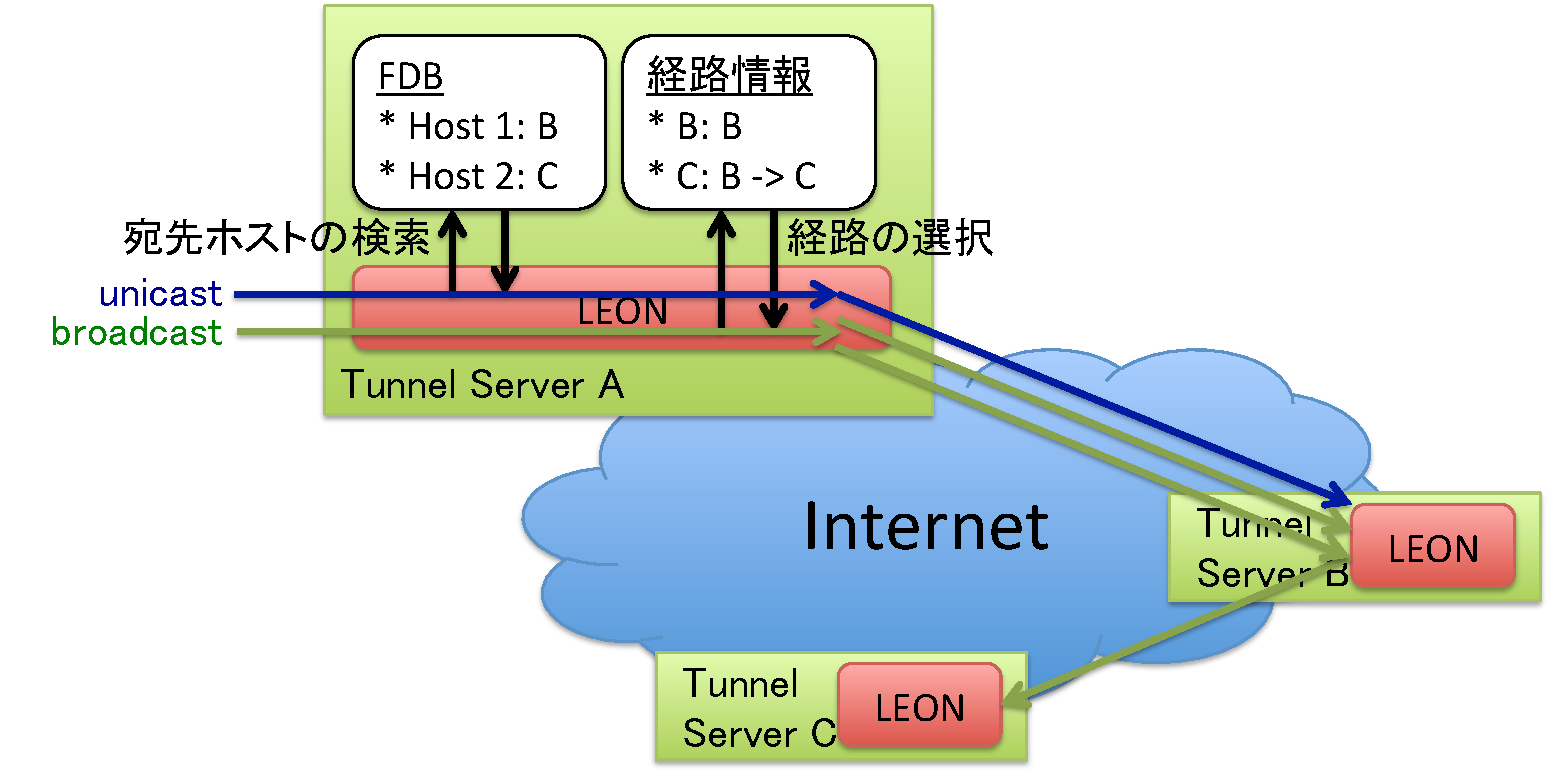
\includegraphics[scale=0.60]{./img/forwardabst}
		\caption{転送動作の概要}
		\label{img:forwardabst}
	\end{center}
\end{figure}

イーサネットフレームの転送は、各トンネル終端点がそれぞれ持つ経路表と自動的に学習された
FDBをもとに、宛先ホストまでの遅延が最も小さい経路で転送される。転送動作の概要を図~\ref{img:forwardabst}
に示す。トンネル終端点が転送
するイーサネットフレームを受け取ると、そのイーサネットフレームがユニキャストフレームか
ブロードキャストフレームかを判別する。ユニキャストフレームの場合、宛先ホストがどの
トンネル終端点によって収容されているかFDBから検索する。そして、経路表に従い、
宛先までの遅延が最も小さい経路で転送するための転送先を決定する。ブロードキャストフレームの場合は、
宛先ホストが所属しているトンネル終端点として全てのトンネル終端点を選択し、それぞれの
トンネル終端点に転送するにあたり、遅延が最も小さい経路で転送するための転送先を決定する。
インターネットの経路で宛先のトンネル終端点に到達することにより、遅延が最も小さく転送できるのであれば、転送先は宛先のトンネル終端点となる。
他のトンネル終端点を中継させることにより、遅延がインターネットの経路で直接転送した時よりも
小さくなるのであれば、転送先は中継するトンネル終端点となる。転送先が決定されると、
イーサネットフレームに転送経路が書かれたヘッダーと転送先のトンネル終端点が宛先となっているIPヘッダー
が追加され、インターネットにエンキャプシュレーションされたイーサネットフレームが転送される。
ユニキャストフレームの場合、転送先が1つなのでエンキャプシュレーション作業は1回のみである。
ブロードキャストフレームの場合、転送先が複数あるので、Layer 2ネットワークに参加しているトンネル終端点
の台数と同じ回数、エンキャプシュレーション作業が行われる。LEONではこのように、遅延が
最も小さい経路で、イーサネットフレームの転送を行う。

トンネル終端点が、エンキャプシュレーションされたイーサネットフレームを受信した際には、
イーサネットフレームに追加されたLEONヘッダーに記述された経路に応じて転送を行う。Layer 2ネットワーク上の
ホストから、他のトンネル終端点によって収容されているホストが宛先であるイーサネットフレームを受信した
トンネル終端点は、そのイーサネットフレームを転送する際に経路表から転送する経路を選択する。選択された経路は、
イーサネットフレームを転送する際に、イーサネットフレームの先頭に追加されるLEONヘッダーに記述される。
そして、トンネル終端点はエンキャプシュレーションされたイーサネットフレームを受け取ると、LEONヘッダー
に記述された経路を確認する。そのトンネル終端点が記述された経路の最後に書かれたトンネル終端点の場合は、その
トンネル終端点宛のイーサネットフレームであると判断し、送信元トンネル終端点によって追加されたIPヘッダー
とLEONヘッダーを取り外し、Layer 2ネットワーク上の宛先ホストへ転送をする。そのトンネル終端点が経路表の最後に書かれた
トンネル終端点でない場合は、そのトンネル終端点の次に記述されているトンネル終端点へイーサネットフレームを
さらに転送する。これにより、トンネル終端点は受信したエンキャプシュレーションされたイーサネットフレームの
転送先を決定する。

これにより、LEONは遅延が最も小さい経路でイーサネットフレームが転送されるLayer 2ネットワークの構築を行う。LEONはLayer 2ネットワーク
に参加しているトンネル終端点間の遅延を計測し、計測結果に基づき、イーサネットフレームの転送先
を選択する。最も遅延が小さくなる経路が、インターネット上の経路に基づいて転送する経路の場合、
インターネット上の経路でイーサネットフレームが転送される。他のトンネル終端点を経由する経路が
遅延の最も小さい経路の場合、経由すべきトンネル終端点に転送される。転送する際に、LEONは
転送経路が記述されたLEONヘッダーをイーサネットフレームに追加する。そして、転送されてきた
イーサネットフレームを受信した際には、LEONヘッダーのイーサネットフレームを参照し、受信した
トンネル終端点が経路の最後に記述されたトンネル終端点の場合は、イーサネットフレームの宛先
ホストへイーサネットフレームを転送する。受信したトンネル終端点が経路の最後に記述されたトンネル
終端点でない場合は、次に記述されているトンネル終端点へ受信したイーサネットフレームを転送する。
これにより、LEONはイーサネットフレームをインターネット上で遅延が最も小さい経路で転送する。

\section{プロトコルの設計}
\label{solv:protocol}

LEONは、遅延が最も小さい経路でイーサネットフレームが転送されるLayer 2ネットワークの構築と利用、そしてトンネル終端点間の遅延を
計測するために大きく分けて3種類のプロトコルを利用する。まず1つ目として、Layer 2ネットワークの
構築を行う際に利用されるコントロールプロトコルである。トンネル終端点は、コントロール
プロトコルを利用して、Layer 2ネットワークへの参加と離脱を行う。2つ目として、イーサネットフレーム
の転送を行う際に利用される転送プロトコルが挙げられる。転送プロトコルを利用して、Layer 2ネットワーク上の
イーサネットフレームがトンネル終端点間でやり取りされる。そして、3つ目として、トンネル終端点間の遅延情報の収集
を行う際に利用される計測プロトコルが挙げられる。計測プロトコルを利用して、トンネル終端点間
の遅延の計測とその計測結果のトンネル終端点間での共有を行う。これらのプロトコルは、全てUDPを
用いる。LEONが用いるメッセージの共通ヘッダーフォーマットを図~\ref{img:mtunheader}に示す。

\begin{figure}[h]
	\begin{center}
		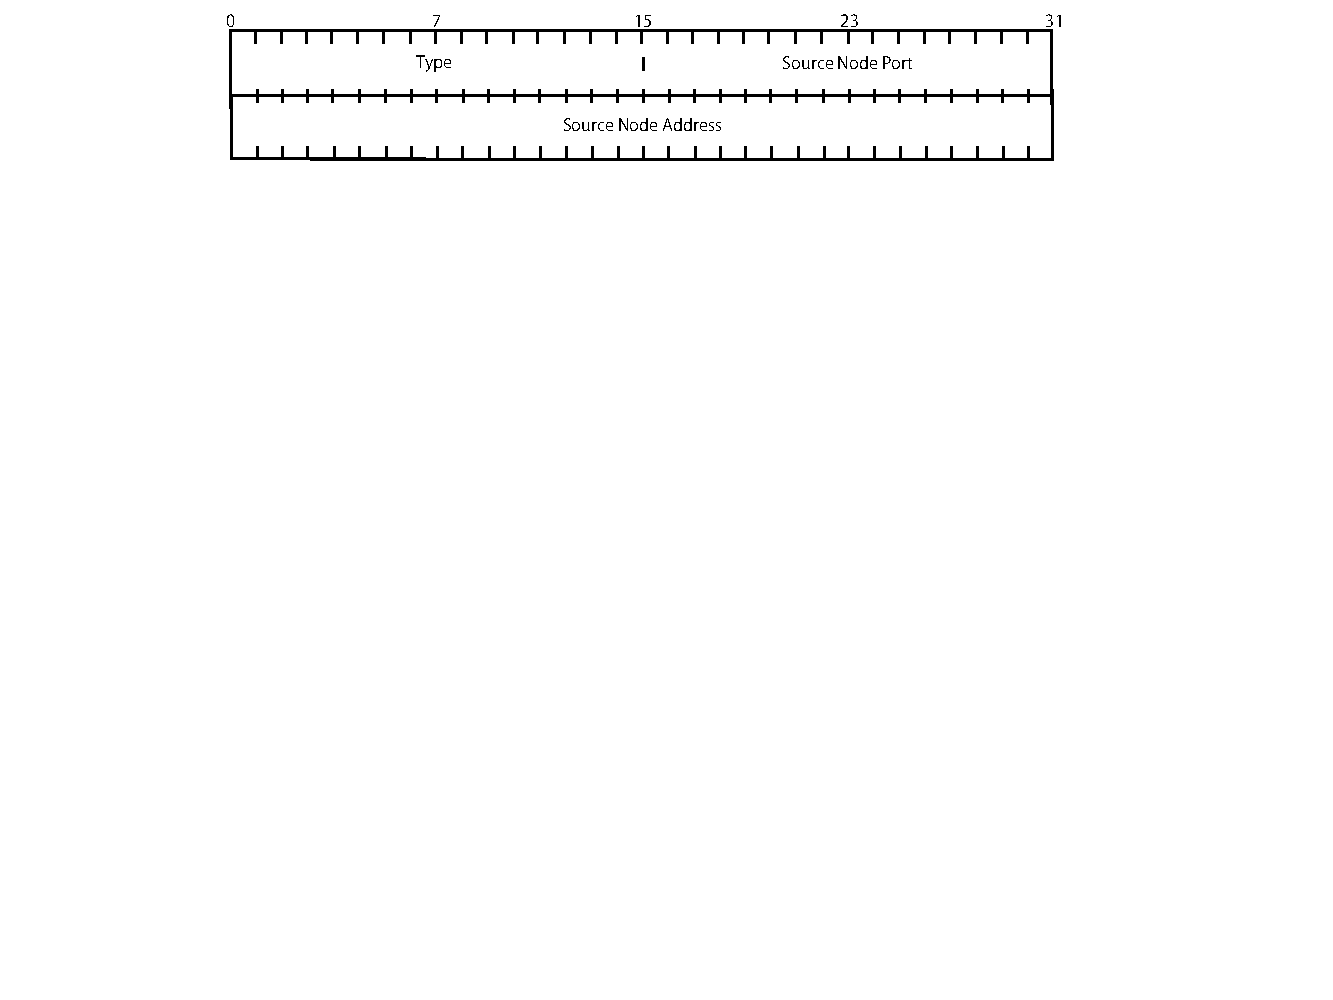
\includegraphics[scale=1.0]{./img/mtunheader}
		\caption{LEONの共通ヘッダーフォーマット}
		\label{img:mtunheader}
	\end{center}
\end{figure}

Typeフィールドは他トンネル終端点から送られてきたメッセージを識別するために利用される。
Typeの種類は全てで8種類である。まず、トンネル終端点がLayer 2ネットワークへ参加と離脱を行うための
コントロールプロトコルで利用されるTypeとしてJOINNODE(20)、JOINNODEACK(21)、DELNODE(30)、REQALL(40)の5種類
がある。次に、トンネル終端点間でイーサネットフレームの転送を行うための転送プロトコルで利用されるTypeとしてFORWARD(10)
の1種類がある。最後に、トンネル終端点間の遅延情報の収集を行うための遅延計測プロトコルで利用されるTypeとしてPINGREQ(50)、
PINGACK(51)、LATENCYDATA(60)の3種類がある。Source Node AddressとSource Node Portフィールドはメッセージの送信元トンネル終端点
のIPアドレスとポート番号が挿入されている。以下に、各プロトコルの詳細について述べる。

\subsection{コントロールプロトコル}
\label{solv:controlprotocol}

コントロールプロトコルはトンネル終端点がLayer 2ネットワークに参加と離脱を行う際に
用いられる。コントロールメッセージのフォーマットを図~\ref{img:controlheader}に示す。

\begin{figure}[h]
	\begin{center}
		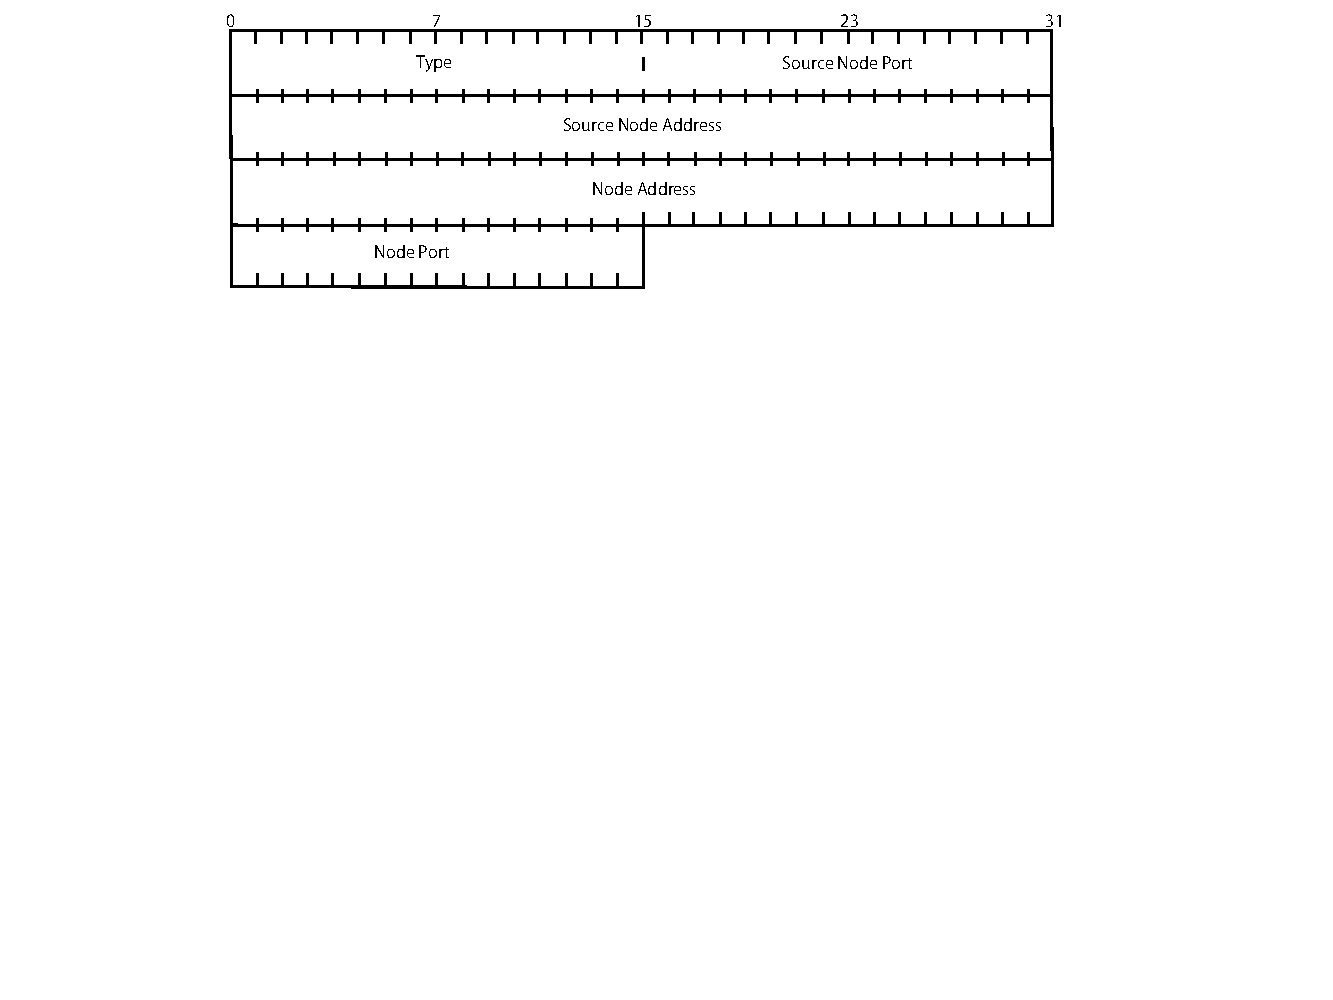
\includegraphics[scale=1.0]{./img/controlmessage}
		\caption{コントロールメッセージのフォーマット}
		\label{img:controlheader}
	\end{center}
\end{figure}

\begin{figure}
	\begin{center}
		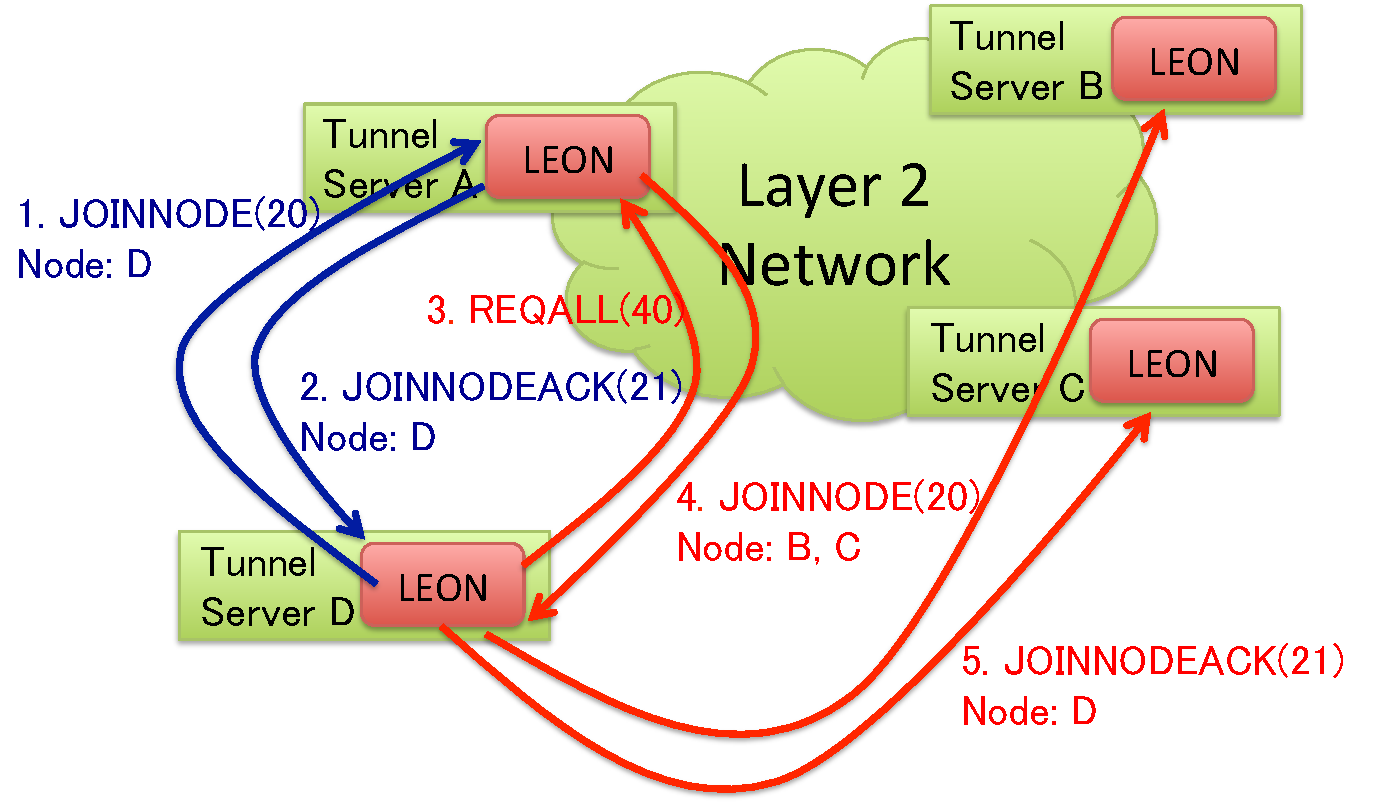
\includegraphics[scale=0.60]{./img/joinnodeproc}
		\caption{新規トンネル終端点の参加プロセス}
		\label{img:joinnodeproc}
	\end{center}
\end{figure}

トンネル終端点が新たに既存のLayer 2ネットワークに参加する際の手順を図~\ref{img:joinnodeproc}に示す。まず、既にLayer 2ネットワークに
参加しているトンネル終端点の1つにTypeフィールドがJOINNODE(20)であるコントロールメッセージを
送信する。このときコントロールメッセージのNode AddressフィールドとNode Portフィールドには、
新たに参加するトンネル終端点のIPアドレスとポート番号が挿入されている。送信された
コントロールメッセージを受信したトンネル終端点は、そのトンネル終端点が管理しているトンネル終端点
一覧に送信元トンネル終端点を追加する。そして、正常に受け取ったことを送信元トンネル終端点に通知するために、
JOINNODEACK(21)となっているコントロールメッセージを送信する。このときコントロールメッセージの
Node AddressフィールドとNode Portフィールドは新たに参加したトンネル終端点のIPアドレスと
ポート番号が挿入されている。新たに参加するトンネル終端点が、JOINNODEACK(21)となっている
コントロールメッセージを受信すると、新たに参加するトンネル終端点が管理するトンネル終端点
一覧に既にLayer 2ネットワークに参加しているトンネル終端点の1つが登録される。次に、新たに参加するトンネル終端点は、
他の既にLayer 2ネットワークに参加しているトンネル終端点に対しても同様な登録作業を行う
必要があるため、登録作業を済ませたトンネル終端点から既に参加している全トンネル終端点の一覧を
取得する。一覧を取得するためには、TypeフィールドがREQALL(40)であるコントロールメッセージ
を送信する。このときコントロールメッセージのNode AddressフィールドとNode Portフィールド
は0である。このコントロールメッセージを受信したトンネル終端点は、TypeフィールドがJOINNODE(20)であるコントロールメッセージ
を全トンネル終端点分送り返す。Node AddressフィールドとNode Portフィールドに既に参加している
各トンネル終端点を挿入し、コントロールメッセージを送信する。新たに参加するトンネル終端点が
このコントロールメッセージを受信すると、自身が管理するトンネル終端点一覧にNode Addressフィールドと
Node Portフィールドに書かれたトンネル終端点を登録する。そして、登録したトンネル終端点に対して、
TypeフィールドがJOINNODEACK(21)であるコントロールメッセージを送信する。これにより、相手のトンネル終端点に
相手が管理しているトンネル終端点一覧に、新たなトンネル終端点の登録をしてもらう。
この手順で新たなトンネル終端点は既存のLayer 2ネットワークに参加する。

\begin{figure}
	\begin{center}
		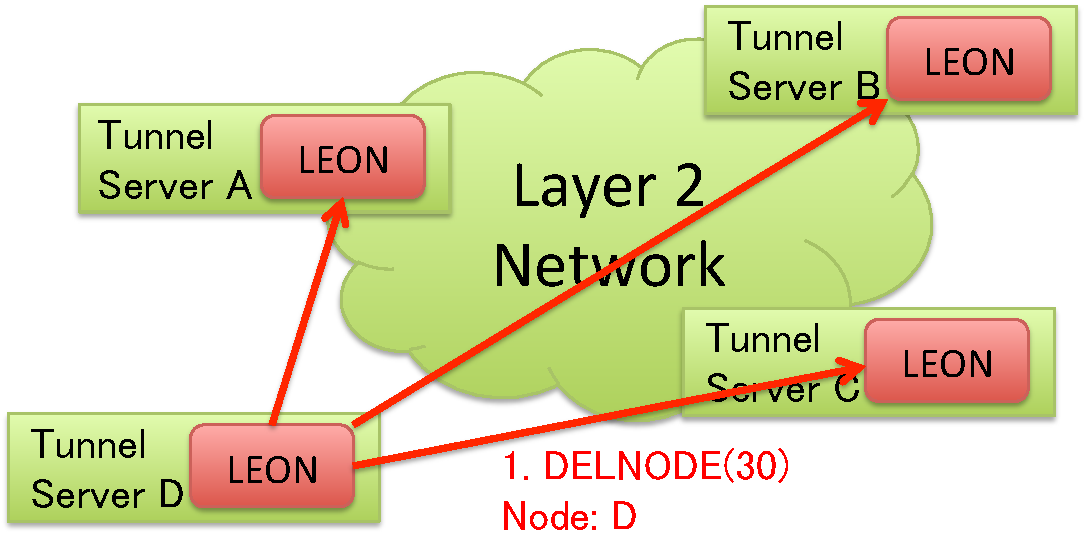
\includegraphics[scale=0.60]{./img/delnodeproc}
		\caption{トンネル終端点の離脱プロセス}
		\label{img:delnodeproc}
	\end{center}
\end{figure}

トンネル終端点が参加しているLayer 2ネットワークを離脱する際の手順を図~\ref{img:delnodeproc}に示す。
離脱するトンネル終端点は、トンネル終端点一覧に入っている
全てのトンネル終端点に対してTypeフィールドがDELNODE(30)であるコントロールメッセージを送信する。
このとき、Node AddressフィールドとNode Portフィールドには離脱するトンネル終端点のIPアドレスと
ポート番号が挿入される。そして、このコントロールメッセージを受信したトンネル終端点は、Node Address
フィールドとNode Portフィールドに挿入されたトンネル終端点をトンネル終端点一覧から削除する。
また、同時に、そのトンネル終端点によって収容されていたホストをFDBから削除する。これにより、
トンネル終端点は参加しているLayer 2ネットワークから離脱される。

\subsection{転送プロトコル}
\label{solv:fowardprotocol}

転送プロトコルはトンネル終端点が受信したイーサネットフレームを転送する際と、トンネル終端点が
イーサネットフレームを中継する際に用いられる。転送メッセージのフォーマットを図~\ref{img:forwardheader}
に示す。

\begin{figure}[h]
	\begin{center}
		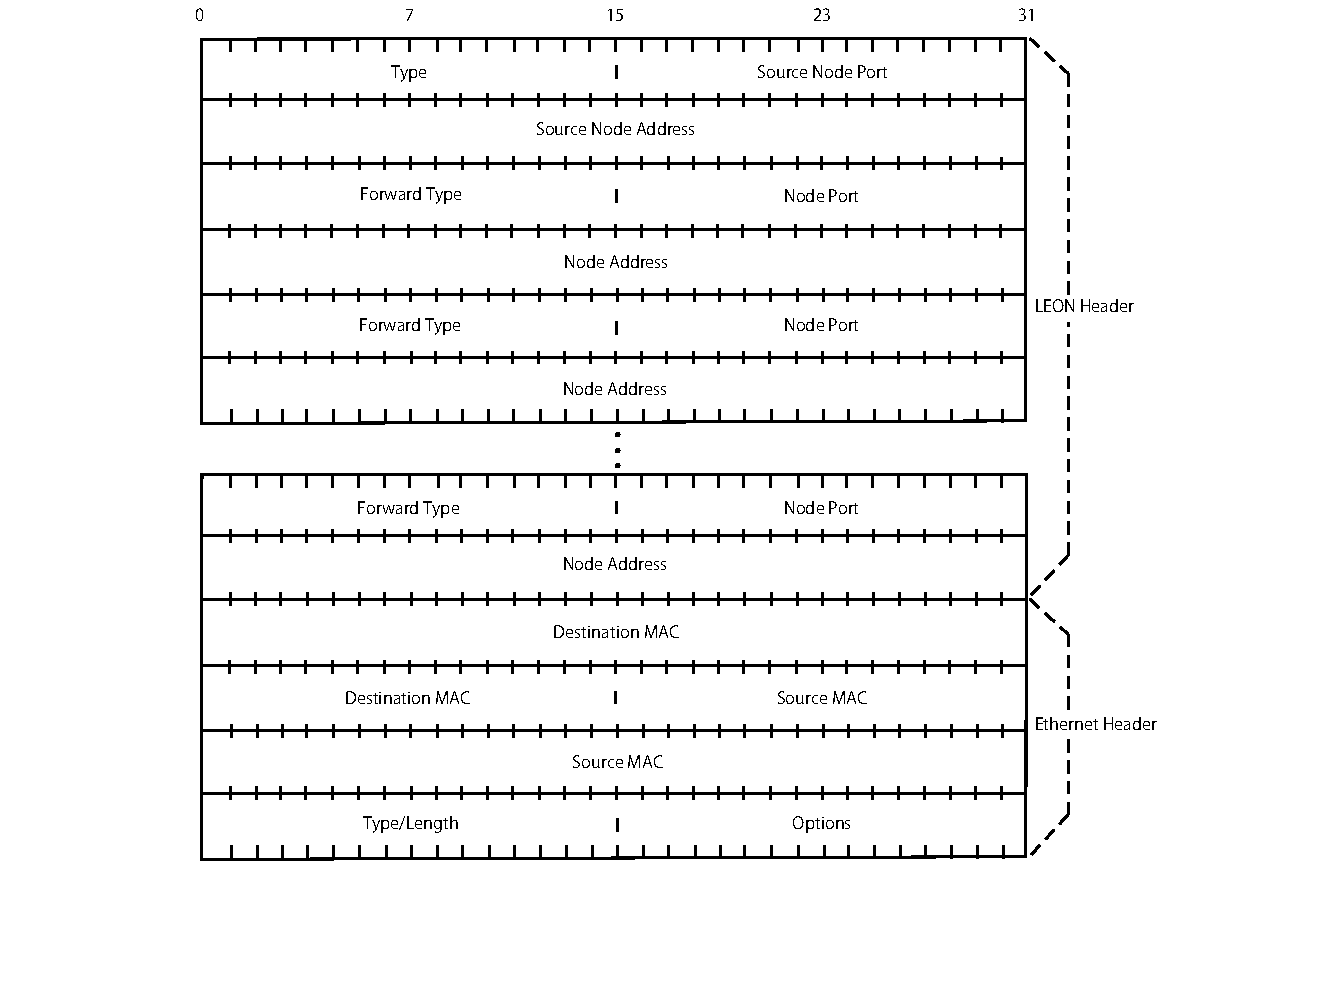
\includegraphics[scale=1.0]{./img/forwardheader}
		\caption{転送メッセージのパケットフォーマット}
		\label{img:forwardheader}
	\end{center}
\end{figure}

転送メッセージはLEONヘッダーとホストから受信したイーサネットフレームによって構成される。LEONヘッダーは
共通ヘッダーと転送経路情報で成り立っている。転送経路情報は転送メッセージを中継するトンネル終端点と
最終的に受信するトンネル終端点のリストである。トンネル終端点は転送メッセージをLEONヘッダーの転送経路情報
に従って転送する。転送メッセージのForward Typeフィールドは、次に書かれたトンネル終端点が中継するための
トンネル終端点か受信するトンネル終端点かを識別するためのものである。Foward TypeフィールドにはFORWARD(1)
またはRECEIVE(0)のどちらかを挿入する。そして、その次のNode Address及びNode Portフィールドには中継、または、
受信をするトンネル終端点のIPアドレスとポート番号を挿入する。転送経路情報の後ろにはホストから受信したイーサネット
フレームを付加する。

\begin{figure}
	\begin{center}
		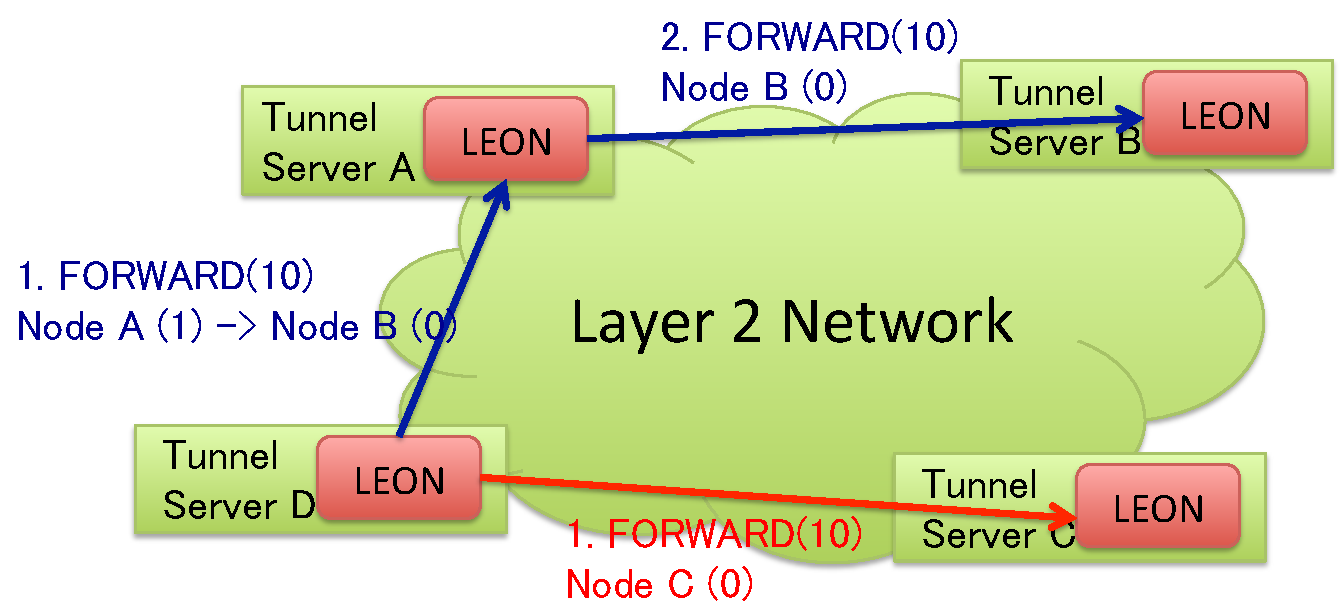
\includegraphics[scale=0.60]{./img/forwardproc}
		\caption{イーサネットフレームの転送プロセス}
		\label{img:fwdproc}
	\end{center}
\end{figure}

トンネル終端点が受信したイーサネットフレームを転送する際の手順を図~\ref{img:fwdproc}に示す。
トンネル終端点が収容しているホストからイーサネットフレームを受信すると、イーサネットフレームの
Destination MACフィールドを参照し、宛先のホストがどのトンネル終端点によって収容されているかFDB
から検索し、そのトンネル終端点までの経路を選択する。そして、イーサネットフレームの先頭にLEONヘッダー
を追加する。この際の共通ヘッダーのTypeフィールドはFORWARD(10)、Source Node AddressフィールドとSource Node Portフィールドは
イーサネットフレームを受信したトンネル終端点のIPアドレスとポート番号である。また、転送経路情報
の部分には選択された経路が挿入される。イーサネットフレームを直接宛先のトンネル終端点に転送する
場合は、転送経路情報はForward TypeフィールドがRECEIVE(0)、Node AddressフィールドとNode Portフィールドが宛先
トンネル終端点のIPアドレスとポート番号の1つである。イーサネットフレームを他のトンネル終端点を
中継して転送する場合は、転送経路情報はForward TypeフィールドがFORWARD(1)、Node Addressフィールドと
Node Portフィールドあ中継するトンネル終端点のIPアドレスとポート番号のヘッダー部分が中継するトンネル終端点
分追加される。そして、その後に最終的に受信するトンネル終端点のヘッダー部分を追加する。このとき追加される
ヘッダー部分は直接転送する場合のヘッダー部分と同じである。最後に、イーサネットフレームが
LEONヘッダーの後ろに追加される。

トンネル終端点が転送メッセージを受信すると自分を転送経路情報から探し、Forward Typeフィールドを
確認する。Forward TypeフィールドがRECEIVE(0)の場合、受信したトンネル終端点が最終的な宛先である
ことがわかる。トンネル終端点はLEONヘッダーを受信したパケットから取り除き、イーサネットフレーム
をLayer 2ネットワーク上の宛先ホストへ転送する。Foward TypeフィールドがFORWARD(1)の場合、受信した
トンネル終端点は中継用のトンネル終端点であることがわかる。トンネル終端点はLEONヘッダーの転送経路情報
から、そのトンネル終端点を転送経路情報からを消去し、次に指定されているトンネル終端点へ転送する。この際、最終的な宛先であるトンネル終端点が
、それがどのトンネル終端点から送信されたものか判別できるよう、共通ヘッダーのSource Node
AddressフィールドとSource Node Portフィールドの変更は行わない。

\subsection{遅延計測プロトコル}
\label{solv:latencyprotocol}

遅延計測プロトコルはトンネル終端点間の遅延の計測と、その計測結果の共有に用いられる。遅延の計測を行うための
遅延計測メッセージのフォーマットを図~\ref{img:ldcmessage}に示す。また、計測結果を共有するための遅延データ
メッセージのフォーマットを図~\ref{img:ldmessage}に示す。


\begin{figure}[h]
	\begin{center}
		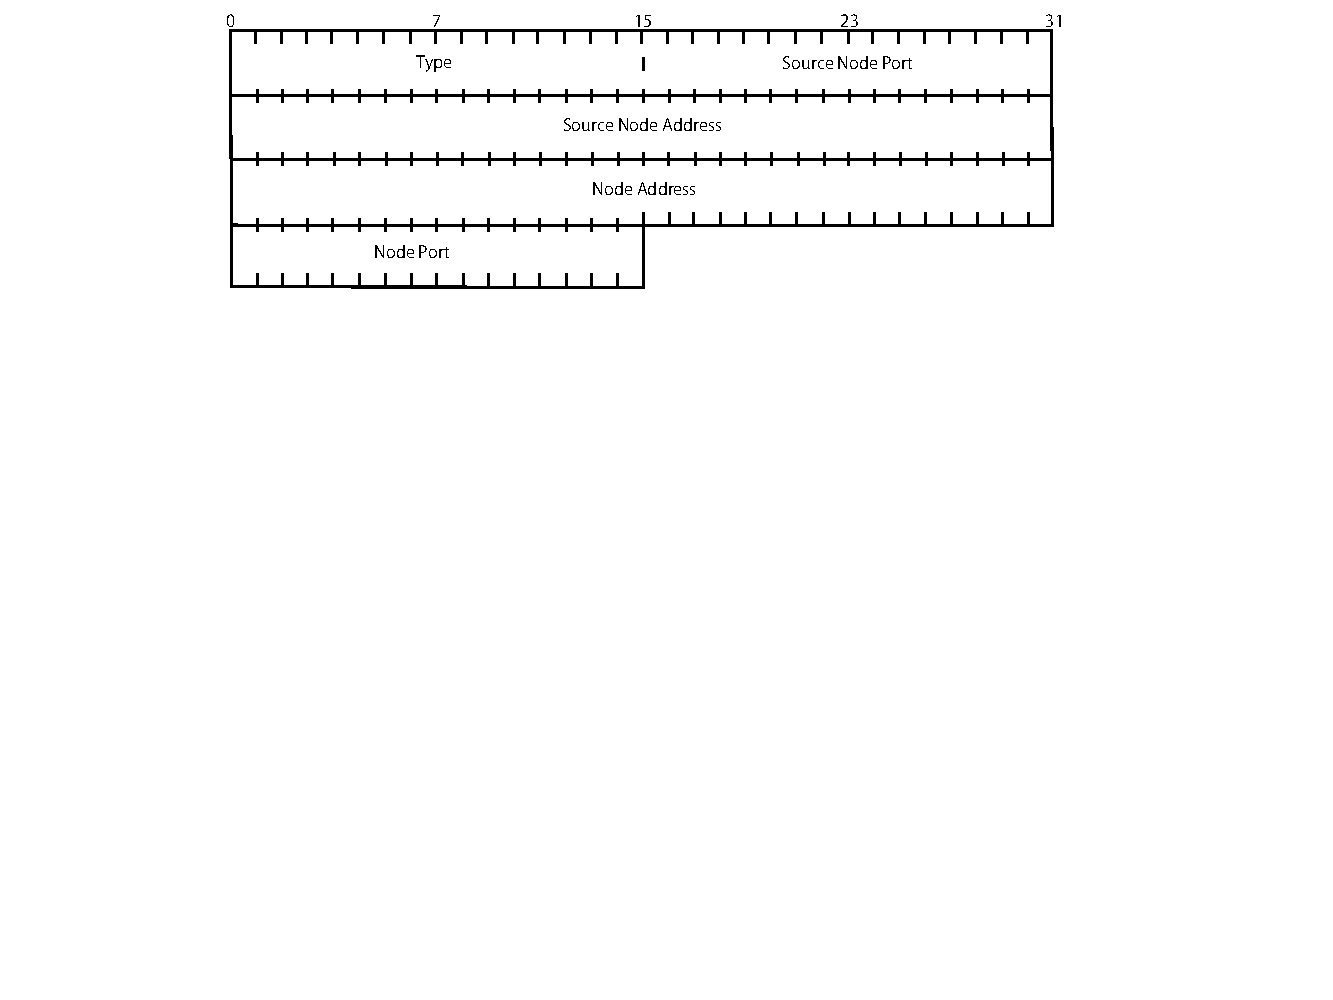
\includegraphics[scale=1.0]{./img/controlmessage}
		\caption{遅延計測メッセージのフォーマット}
		\label{img:ldcmessage}
	\end{center}
\end{figure}

\begin{figure}[h]
	\begin{center}
		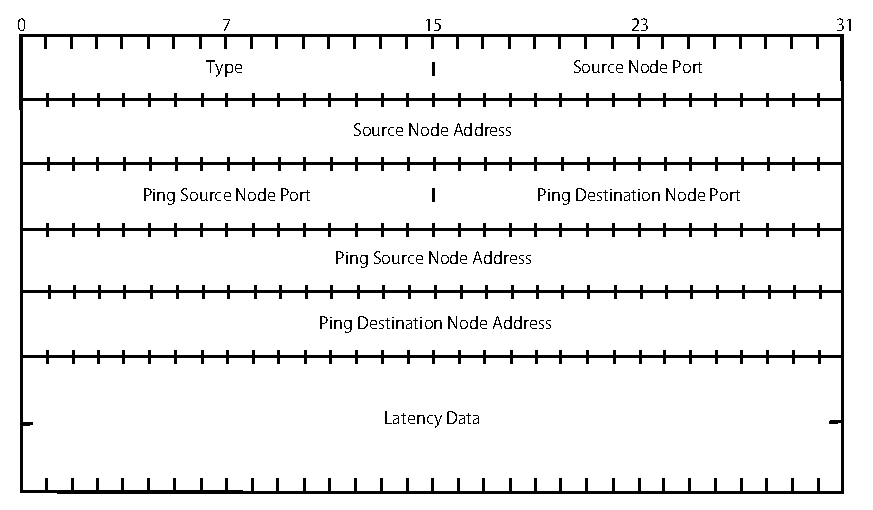
\includegraphics[scale=1.0]{./img/latencydatamessage}
		\caption{遅延データメッセージのフォーマット}
		\label{img:ldmessage}
	\end{center}
\end{figure}

\begin{figure}
	\begin{center}
		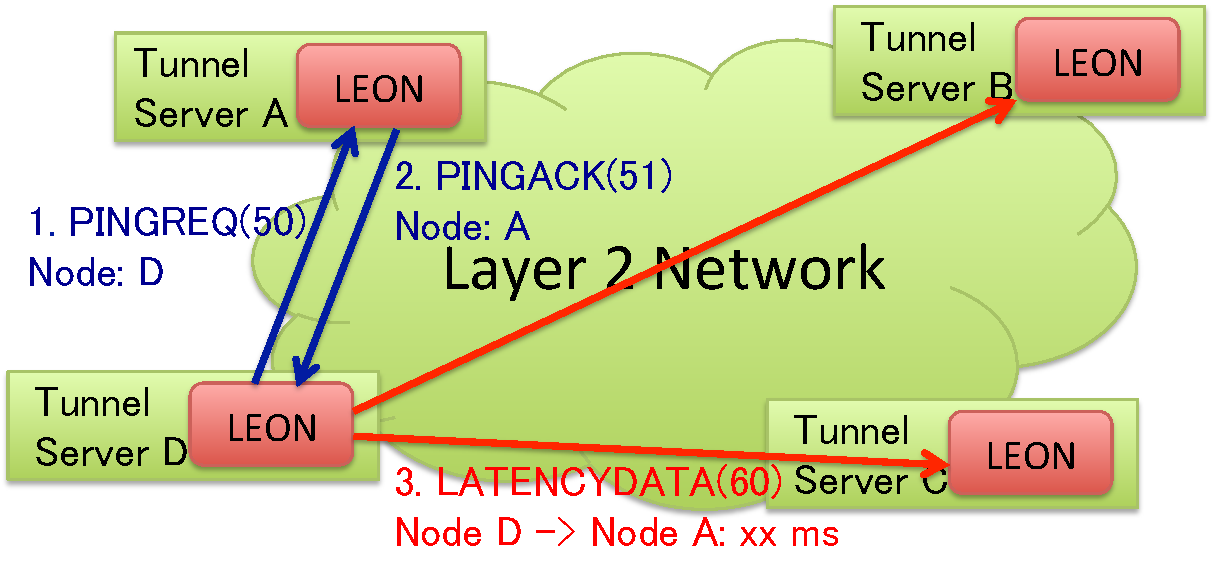
\includegraphics[scale=0.60]{./img/latencyproc}
		\caption{遅延データの共有プロセス}
		\label{img:ldproc}
	\end{center}
\end{figure}

トンネル終端点がトンネル終端点間の遅延を計測し、その計測結果を共有する際の手順を図~\ref{img:ldproc}
に示す。トンネル終端点間の遅延計測は定期的に全トンネル終端点で行われる。まず、トンネル終端点は
トンネル終端点が管理するトンネル終端点一覧に登録されている全トンネル終端点までの遅延を計測する。
遅延の計測を行うには、トンネル終端点は宛先のトンネル終端点に遅延計測メッセージを送信する。
遅延計測メッセージのTypeフィールドにはPINGREQ(50)、Source Node Addressフィールド、Node Addressフィールド
Source Node PortフィールドとNode Portフィールドには遅延計測を行うトンネル終端点のIPアドレスとポート番号を
挿入する。また、遅延計測を行うトンネル終端点は遅延計測メッセージの送信した時間を記憶する。そして、
遅延計測メッセージを受信したトンネル終端点は同様に遅延計測メッセージを返す。この時の遅延計測メッセージ
のTypeフィールドにはPINGACK(51)、Source Node Addressフィールド、Node Addressフィールド、Source Node Portフィールド
とNode Portフィールドには返信をするトンネル終端点のIPアドレスとポート番号を挿入する。遅延計測を行うトンネル終端点
が返信の遅延計測メッセージを受け取ると、受け取った時間から送信した時間の差から遅延を求める。そして、遅延を
遅延データベースに登録する。

また、トンネル終端点間の遅延計測結果は各トンネル終端点が経路選択を行う際に必要となる。そのため、
トンネル終端点は遅延計測結果を遅延データベースに登録後、遅延結果をトンネル終端点一覧に登録されて
いる全トンネル終端点に通知する。通知には遅延データメッセージが用いられる。遅延データメッセージには
遅延計測メッセージの送信元と送信先、及び、遅延の計測結果が含まれる。共通ヘッダー部分のTypeフィールド
にはLATENCYDATA(60)、Source Node AddressとSource Node Portフィールドには遅延データメッセージを送信
するトンネル終端点のIPアドレスとポート番号を挿入する。遅延データ部分のPing Source Node Addressフィールド
とPing Source Node Portフィールドには遅延計測メッセージを送信したトンネル終端点のIPアドレスとポート番号、
Ping Destination Node PortフィールドとPing Destination Node Addressフィールドには遅延計測メッセージを受信した
トンネル終端点のIPアドレスとポート番号、Latency Dataフィールドには遅延の計測結果を挿入する。この遅延データ
メッセージを受信したトンネル終端点は遅延データベースに指定されたトンネル終端点間の遅延データを登録する。
そして、収集された遅延データを用いて遅延が最も小さい経路を選択する。

\section{実装}
\label{solv:coding}

本節では、LEONの実装について述べる。本節では、本実装のことをleondと呼ぶ。

\subsection{実装環境}
\label{solv:codeenv}

表~\ref{table:codingenv}に本提案手法を実装するにあたり、利用した環境を示す。

\begin{table}[h]
	\begin{center}
		\caption{実装環境}
		\begin{tabular}{|l|l|}
			\hline
			CPU & Intel Xeon L5520 2.27Ghz * 2 (8 Cores) \\
			\hline
			RAM & 24GB DDR3 RAM \\
			\hline
			NIC & Intel 82575EB Gigabit NIC \\
			\hline
			使用OS & Debian 6.0.6 Squeeze \\
			\hline
			使用カーネル & Linux Kernel 3.7.2 \\
			\hline
			使用言語 & C言語 \\
			\hline
		\end{tabular}
		\label{table:codingenv}
	\end{center}
\end{table}

\subsection{実装概要}
\label{code:abst}

表~\ref{table:leonmods}にleondの各機構を構成するモジュールを示す。また、各モジュール間の関
係について図~\ref{img:leonoverview}に示す。

\begin{table}[h]
\begin{center}
	\caption{leondのモジュール}
	\begin{tabular}{|l|l|}
		\hline
		機構 & モジュール \\
		\hline
		\hline
		フレーム転送機構 & main\_poller \\
		終端点管理機構   & \\
		\hline
		遅延計測機構     & pinger \\
		\hline
		トポロジ構築機構 & topology \\
		\hline
		経路表 & fdb  \\
		       & nodelist \\
		\hline
	\end{tabular}
	\label{table:leonmods}
\end{center}
\end{table}

\begin{figure}
	\begin{center}
		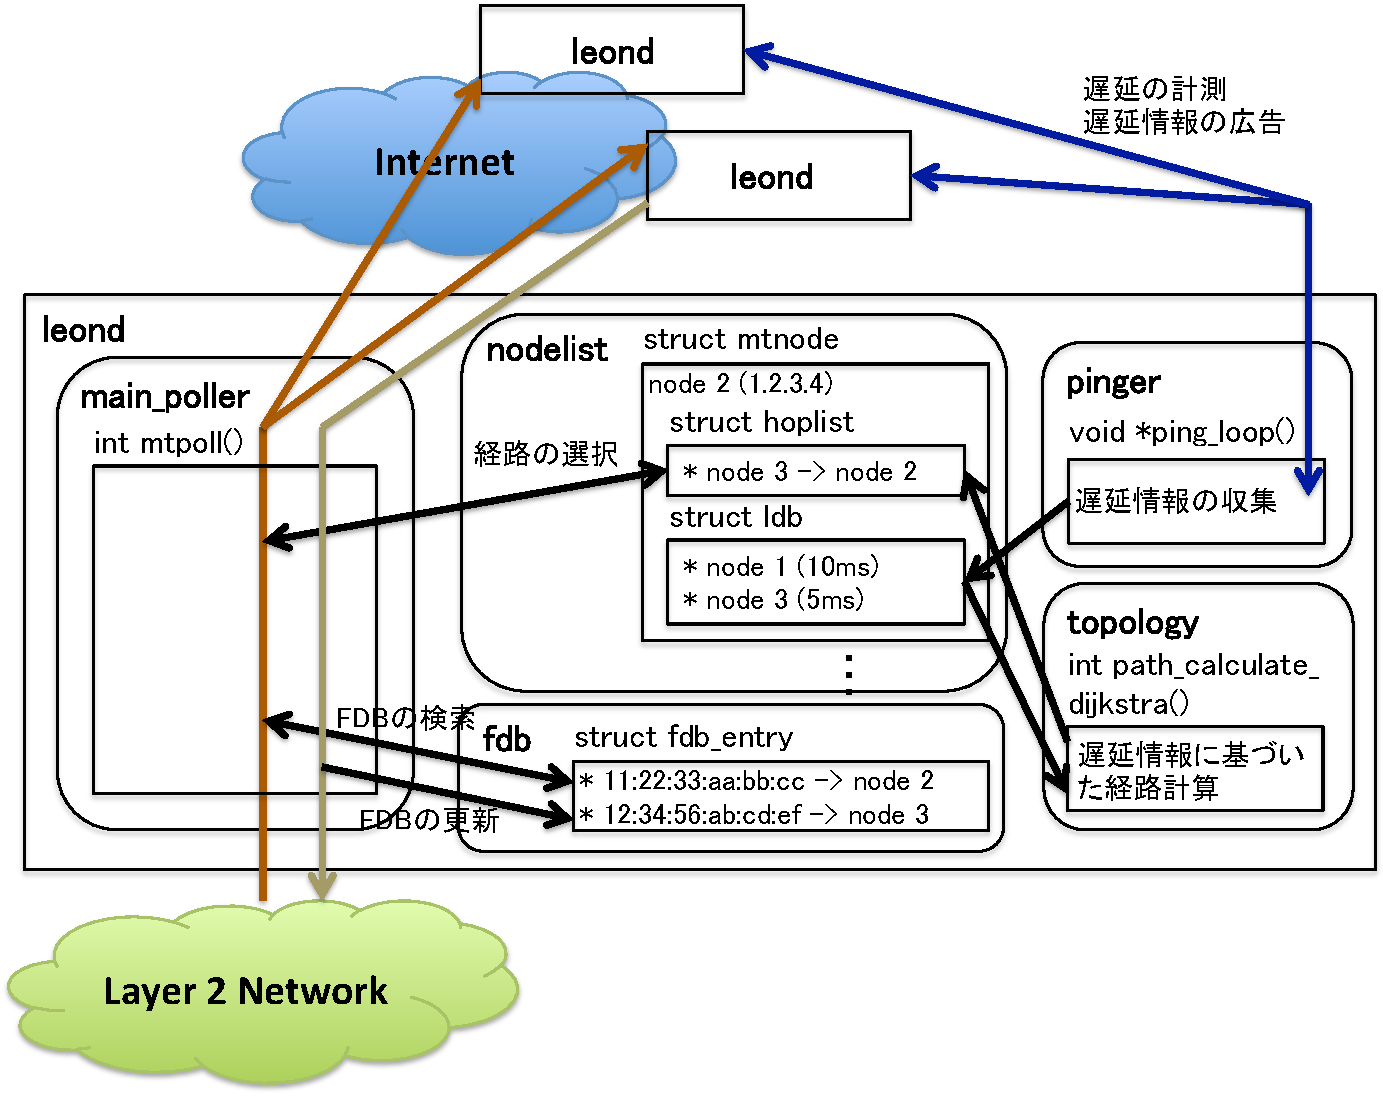
\includegraphics[scale=0.70]{./img/leonoverview}
		\caption{leondのモジュール間の関係}
		\label{img:leonoverview}
	\end{center}
\end{figure}

leondの引数と起動例を下記に示す。

\begin{verbatim}
$ ./leond
--debug: debug mode
-d: run as daemon
-u: localaddr:port
-p: peeraddr:port
--ping-interval: ping interval seconds

$ ./leond -d -u 1.2.3.4:10000 (既存のLayer 2ネットワークに参加しない場合)
$ ./leond -d -u 5.6.7.8:10000 -p 1.2.3.4:10000 (既存のLayer 2ネットワークに参加する場合)
\end{verbatim}

leondを起動するにあたり、必須である引数は\texttt{-u}オプションのみである。\texttt{-u}オプションには他のトンネル終端点からの
通信を待ち受けるために利用するIPアドレスとポート番号を指定する。また、既に他のトンネル終端点によって拡張
されているLayer 2ネットワークに参加する際には、既に参加しているトンネル終端点のIPアドレスとポート番号を
\texttt{-p}オプションで指定する。

また、遅延の計測を行う間隔のデフォルト値は60秒にした。デフォルト値から変更したい場合は、\texttt{--ping-interval}
オプションで遅延を計測する間隔を秒単位で指定することにより変更が可能である。デフォルト値を60秒に設定した理由は、
遅延の計測を小さい間隔で行うと、遅延データメッセージと遅延計測メッセージが大量に発生してしまう可能性があったからである。
Layer 2ネットワークに参加しているトンネル終端点の台数を$ N $、1回の遅延計測で発生するメッセージ数を$ M $とし、この2つの関係を数式で表すと次のようになる。

\begin{displaymath}
\displaystyle M = (2 + N) \times N
\end{displaymath}

そのため、例えば30台のトンネル終端点で、遅延計測の間隔を30秒とすると、30秒間で$ M = (2 + 30) \times 30 = 960 $個のメッセージが発生する。
この内、1台のトンネル終端点が処理するメッセージの量は$ 960 \div 30 = 32 $個である。32個のメッセージを30秒で処理するためには、トンネル終端点
は1秒に1個以上処理する必要がある。これではトンネル終端点が高負荷状態となり、イーサネットフレームの転送に遅延が発生する可能性があったので、
遅延計測の間隔を60秒とした。30台のトンネル終端点で、遅延計測の間隔が60秒の場合、トンネル終端点はメッセージを2秒に1個以上処理すれば良い。

\subsection{遅延計測機構}
\label{solv:latency}

遅延計測機構はpingerモジュールによって構成されている。pingerモジュールは、トポロジー構築機構に他トンネル終端点
にイーサネットフレームを転送するための経路を計算する際に必要となる情報を提供する。pingerモジュールの機能は3つある。
以下にそれぞれについて述べる。

まず1つ目のpingerモジュールの機能として、遅延データベースの管理が挙げられる。leondを利用して拡張されたLayer 2ネットワークに参加している
トンネル終端点の情報は、後述するnodelistモジュールが提供する\texttt{mtnode}構造体に記憶されている。\texttt{mtnode}構造体は参加している
トンネル終端点に対して1つ存在する。pingerモジュールは\texttt{mtnode}構造体の内部にある、\texttt{ldb}構造体の管理を行う。\texttt{ldb}構造体には
トンネル終端点間の遅延情報が記憶されている。pingerモジュールは遅延の計測結果、及び、他トンネル終端点から広告された
遅延情報を利用し\texttt{ldb}構造体の更新を行う。

2つ目のpingerモジュールの機能として他トンネル終端点までの遅延計測が挙げられる。遅延計測機能は起動時に\texttt{--ping-interval}オプションによって指定された時間毎
に呼び出される。起動時に指定されなかった場合は60秒毎に呼び出される。遅延計測機能が呼び出されると、~\ref{solv:latencyprotocol}項で説明した、
遅延計測メッセージを拡張されたLayer 2ネットワークに参加している全てのトンネル終端点に送信する。そして、他トンネル終端点から送信した遅延計測メッセージ
の返答を受け取ると、送信してから返信を受け取るまでに経過した時間を計算し、その時間を遅延として遅延データベースに登録する。また、遅延情報は
他のトンネル終端点が経路計算を同様に行うために必要となるため、全てのトンネル終端点に遅延情報を~\ref{solv:latencyprotocol}項で説明した、遅延データメッセージ
を用いて広告する。遅延データメッセージを受信したトンネル終端点は同様に、遅延情報を遅延データベースに登録する。

そして3つ目のpingerモジュールの機能として、トンネル終端点の死活監視が上げられる。
あるトンネル終端点から遅延計測メッセージの返信がない場合、そのトンネル終端点の遅延計測失敗回数を増加させる。失敗回数が2回になると、
そのトンネル終端点で障害が発生したと判断し、そのトンネル終端点をトンネル終端点リストから消去する。そして、トポロジー構築機構を呼び出し、
経路の再計算を行う。遅延計測失敗回数は、トンネル終端点から返信を受け取ると0に戻る。


\subsection{トポロジー構築機構}
\label{solv:dijkstra}

トポロジー構築機構はtopologyモジュールによって構成される。topologyモジュールは、leondを利用して拡張されたLayer 2ネットワークに参加している全てのトンネル終端点までの遅延が最も小さい
経路を計算する。フレーム転送機構はtopologyモジュールによって計算された経路を基に、イーサネットフレーム
の転送を行う。

topologyモジュールはpingerモジュールの遅延計測機能が呼び出された後に呼び出される。topologyモジュールが呼び出されると、
pingerモジュールによって収集された遅延データベースを基にダイクストラ法を用いて、トンネル終端点から拡張された
Layer 2ネットワークに参加している全てのトンネル終端点までの遅延が最も小さい経路の計算を行う。そして、
経路はフレーム転送機構が利用できるように、\texttt{mtnode}構造体の内部にある\texttt{hoplist}構造体に記憶する。topologyモジュールは
計算した経路を、経由するトンネル終端点の\texttt{mtnode}構造体へのポインターを、\texttt{hoplist}構造体に経由する順番通りにリスト構造状で
記憶する。

\subsection{経路表}
\label{solv:transfer}

経路表はfdbモジュールとnodelistモジュールによって構成される。nodelistモジュールは同一の拡張されたLayer 2ネットワークに参加している
トンネル終端点の情報を管理する。トンネル終端点の情報はnodelistモジュールが管理する\texttt{mtnode}構造体に格納される。\texttt{mtnode}構造体にはトンネル
終端点のIPアドレスとポート番号、遅延データベースである\texttt{ldb}構造体へのポインターとトンネル終端点へイーサネットフレームへ転送するための
経路情報が記憶されている\texttt{hoplist}構造体へのポインターが格納されている。他のモジュールがトンネル終端点の情報の追加や削除、検索を行う際には、
nodelistモジュールが提供するAPIを利用する。

また、fdbモジュールは拡張されたLayer 2ネットワーク内の各ホストがどのトンネル終端点によって収容されているかを学習する。fdbモジュールは
他のトンネル終端点から転送されたイーサネットフレームを受信した際に呼び出される。fdbモジュールが呼び出されると受信したイーサネットフレーム
の送信元ホストの\texttt{fdb\_entry}構造体が存在するか検索する。\texttt{fdb\_entry}構造体が存在しない場合は、新しい\texttt{fdb\_entry}構造体を作成し、その送信元ホスト
と転送したトンネル終端点の\texttt{mtnode}構造体へのポインターを記憶する。\texttt{fdb\_entry}構造体が存在する場合は、情報の更新が必要か確認し、必要の場合は更新
を行う。また、fdbモジュールは他のモジュールから\texttt{fdb\_entry}構造体の検索、更新、作成を行うためのAPIを提供する。フレーム転送機構がイーサネットフレーム
の転送を行う際には、fdbモジュールが提供するAPIを利用する。

\subsection{フレーム転送機構と終端点管理機構}
\label{solv:join}

フレーム転送機構と終端点管理機構はmain\_pollerモジュールによって構成されている。main\_pollerモジュールは他トンネル終端点
から受信した通信の処理、及び、トンネル終端点が収容しているホストから受信したイーサネットフレームの転送処理といった外部
からのイベント処理を行なっている。main\_pollerモジュールはLinuxのI/Oイベント通知機能であるepollを利用しイベントを待ち受ける。
そして、イベントが発生するとmail\_pollerモジュールの処理が開始する。

発生したイベントがトンネル終端点が収容しているホストからのイーサネットフレーム受信である場合、イーサネットフレームの転送処理
を行う。収容しているホストからイーサネットフレームを受信すると、イーサネットフレームの判別を行う。イーサネットフレームが
ブロードキャストフレームの場合は、全てのトンネル終端点に受信したイーサネットフレームを転送する。ユニキャストフレームの
場合は、送信先ホストをfdbモジュールが提供しているAPIを利用して検索し、転送先のトンネル終端点を決定する。そして、nodelist
モジュールが管理している\texttt{mtnode}構造体内の\texttt{hoplist}構造体に従って、~\ref{solv:fowardprotocol}項で説明した転送メッセージ
のパケットを生成する。最後に、生成した転送メッセージを\texttt{hoplist}構造体の一番最初に指定されているトンネル終端点へ転送する。

発生したイベントが他のトンネル終端点からの通信の場合、まず受信したメッセージの判別を行う。受信したメッセージが
転送メッセージの場合、転送メッセージの転送経路情報を確認する。受信した転送メッセージが自身宛の転送メッセージの場合は、
それを宛先ホストが収容されているLayer 2ネットワークへ転送する。それ以外の場合は、転送経路情報で指定されたトンネル終端点
へ転送メッセージを転送する。また、受信したメッセージがトンネル終端点の参加や離脱などを行うために利用されるコントロールメッセージの場合は、
nodelistモジュールが提供するAPIを利用し、nodelistモジュールの\texttt{mtnode}構造体を更新する。

%%% Local Variables:
%%% mode: japanese-latex
%%% TeX-master: "../yummy_bthesis"
%%% End:

\chapter{評価}
\label{experiment}

本章では、本研究の提案手法であるLEONの評価を行う。

\section{評価方針}
\label{applicationperformance}

~\ref{solv:requirements}節で示した通り、機能要件は、1. インターネット上に分散された複数の拠点へのLayer 2ネットワークの拡張、
2. 宛先に応じた転送先の選択、3. 遅延の最も小さい経路でのイーサネットフレームの転送、4. 分散して動作すること、の4つである。機能要件に
ついて、LEONと~\ref{rw:pointtopoint}節と~\ref{rw:pointtomulti}節で挙げた既存研究が、どの程度満たしてるかを表~\ref{table:relatedworksandleon}
に示す。

\begin{table}[h]
	\begin{center}
		\caption{LEONと既存研究の比較}
		\begin{tabular}{|l|c|c|c|c|}
			\hline
			機能要件 & GRE/L2TP & VXLAN & N2N & LEON \\
			\hline
			\hline
			1. インターネット上の複数環境への拡張 & × & × & ◯ & ◯ \\
			\hline
			2. 宛先に応じた転送先の選択 & × & ◯ & ◯ & ◯ \\
			\hline
			3. 遅延の最も小さい経路での転送 & × & × & × & ◯ \\
			\hline
			4. 分散して動作する & × & ◯ & × & ◯ \\
			\hline
		\end{tabular}
		\label{table:relatedworksandleon}
	\end{center}
\end{table}

GREやL2TPなどといった一対一型のLayer 2ネットワーク拡張技術は、どの機能要件も満たしていない。
一方、VXLANとN2Nは一対多型のLayer 2ネットワーク拡張技術のため、両者共に機能要件の2は満たしている。しかし、両者共に遅延の最も小さい経路でイーサネット
フレームを機能を転送する機能がないため、機能要件の3を満たしていない。インターネット上に分散した複数の拠点にLayer 2ネットワークを拡張するLEONは、
トンネル終端点間の遅延を計測し、計測結果から遅延の最も小さい経路を計算することができる。そして、イーサネットフレームを転送する際に、遅延の最も
小さい経路で転送することができる。そのため、機能要件の1、2、3を満たす。また、N2NはSupernode
を必要とするため、機能要件の4を満たさない。VXLANとLEONは分散して動作するため、機能要件の4を満たす。
以上より、LEONは機能要件を全て満たしている。

LEONはインターネット上に分散した複数の拠点を用いて展開されたサービスのパフォーマンスを向上させることを目標としている。
これを実現するために、LEONはLayer 2ネットワークのイーサネットフレームを遅延の最も小さい経路で転送をする。これにより、
サービスを構成するコンポーネントの通信パフォーマンスが向上し、サービスのパフォーマンスが向上すると予想される。そこで
本研究では、LEONが与えるサービスのパフォーマンスへの影響を評価する。

しかし、一方でLEONは全てのトンネル終端点が、全てのトンネル終端点までの遅延計測や死活監視を行なっている。また、ブロードキャストフレーム
やコントロールメッセージを全てのトンネル終端点に転送する。そのため、トンネル終端点の台数が増加するとLEONに悪影響を与える
と予想される。そこで本研究では、トンネル終端点の増加がLEONに与える影響の評価も行う。

\section{サービスのパフォーマンス}

本研究ではまず、LEONが遅延の最も小さい経路でイーサネットフレームを転送することによって、サービスのパフォーマンス
に与える影響を評価する。本評価を行うにあたり、インターネット上に分散された複数の拠点を用いて構築されたサービス
の例としてWIDE Cloudを用いる。

WIDE Cloudには、~\ref{wcclatency}項で説明したように、複数の拠点でサービスを構築
した場合、コンポーネントのパフォーマンスが低下するためサービスのパフォーマンスが低下してしまうという問題がある。
低下するパフォーマンスの1つとして、仮想マシンのディスクパフォーマンスの低下が挙げられる。
LEONを利用することにより、ストレージとの通信を行う際の遅延が小さくなるため、ストレージのパフォーマンスが改善されると予想される。
これによって仮想マシンのディスクパフォーマンスが改善されると予想される。

本評価を行うにあたり、以下の2点の計測項目を評価に用いる。

\begin{itemize}
	\item{NFSv3のファイルシステムパフォーマンス}
	\item{仮想マシン内でのLinux Kernelコンパイル所要時間}
\end{itemize}

LEONは遅延の最も小さい経路でイーサネットフレームの転送を行う。そのため、直接通信を行った場合と比べ、LEONを利用した場合の方が
小さい遅延でNFSv3の通信を行うことができる。これにより、NFSv3のパフォーマンスは直接通信した場合とLEONを利用した場合と比べると、
LEONを利用した場合の方がファイルシステムのパフォーマンスが良いと予想される。本評価では、この予想が正しいかを知るため、NFSv3の
パフォーマンスを直接通信行った場合とLEONを利用した場合で計測し、これを評価をするための1つの指標とする。

また、NFSv3のパフォーマンスが改善されることにより、仮想マシンのパフォーマンスも改善させると予想される。そこで、
本評価では同様に、NFSv3の通信を直接行った場合とLEONを利用した場合で、仮想マシン内でのLinux Kernel~\cite{linuxkernel}コンパイルにかかる
時間を計測する。そして、これを評価をするための1つの指標とする。

\subsection{実験環境}
\label{spexpenv}

評価を行うにあたり、Layer 2ネットワーク上で動作するサービスとそれを構成するコンポーネントのパフォーマンスを計測する。
この計測を行うにあたって、実験環境に対して以下の要求が受けられる。

\begin{itemize}
	\item{実インターネットでの計測環境}
	\item{直接通信するよりも小さい遅延で通信することができる経路が存在すること}
\end{itemize}

LEONはインターネット上に分散された複数の拠点に同一のLayer 2ネットワークを拡張するために利用される。このような想定環境で構築された
サービスのパフォーマンスに与える影響を計測するため、本研究では実験環境を実インターネット上に構築し計測を行う。また、本研究では、最も小さい
経路でイーサネットフレームを転送することによる影響を計測するため、実験環境には直接通信するより、他の拠点を経由することにより
小さい遅延で通信することができる経路が存在する必要がある。

\begin{figure}
	\begin{center}
		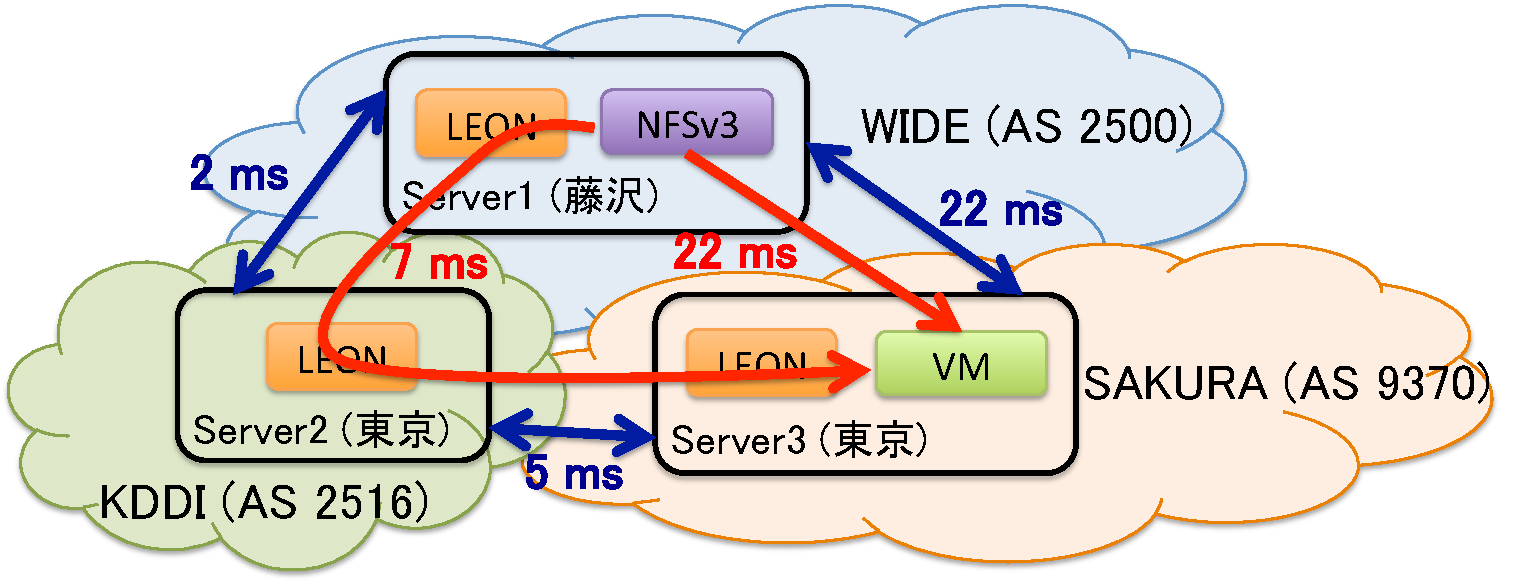
\includegraphics[scale=0.65]{./img/spexp}
		\caption{サービスパフォーマンス計測に用いた実験環境}
		\label{img:spexp}
	\end{center}
\end{figure}

実験環境に対する要求から、本実験を行うにあたり、インターネット上に分散された3つの拠点に設置された3台のサーバーを利用して実験環境を構築した。
この実験環境のトポロジー図を図~\ref{img:spexp}に示す。また、利用した実機サーバーの仕様を表~\ref{table:spserv}に示す。
更に、それぞれのサーバーで利用したソフトウェアのバージョンを表~\ref{table:spversion}に示す。Server 1はWIDE Projectの藤沢NOCに設置されたサーバーである。
Server 2はKDDIウェブコミュニケーションズ社~\cite{kddiwebcom}が提供しているCloudCore VPSサービス~\cite{cloudcore}を利用した
仮想サーバーである。そして、Server 3はEditNet社~\cite{editnet}による
フレッツ光ネクスト接続サービス~\cite{enflets}~\cite{nttflets}を用いて接続されたサーバーである。
EditNet社のサービスはさくらインターネット社~\cite{sakurainc}のバックボーンを利用している~\cite{enbb}。

実験を行うにあたり、これら3台のサーバーでLEONの実装であるleondを動作させた。WIDE Projectとさくらインターネットは堂島でピアリングを行なっている。
そのため、Server 1とServer 3が直接通信した場合、堂島を経由するために遅延が22 ms以上かかる。一方、WIDE ProjectとKDDIは東京でピアリングを行なっている。
また、KDDIとさくらインターネットも同様に、東京でピアリングを行なっている。そのため、Server 1とServer 3が通信を行うにはServer 2を経由することにより、
直接通信した場合よりも小さい遅延で通信をすることができる。leondはこの経路を自動的に発見し、Server 1からServer 3宛のイーサネットフレームを転送する際には
Server 2を経由させ転送をする。

\begin{table}[h]
\begin{center}
	\caption{サービスパフォーマンス計測に用いたサーバーの仕様}
	\begin{tabular}{|l|l|l|l|}
		\hline
		ホスト & CPU & メモリー & NIC \\
		\hline
		\hline
		Server 1 (藤沢) & Intel Xeon L5520 2.27GHz & 12GB & NetXtreme II BCM5709 \\
		\hline
		Server 2 (東京) & AMD Phenom 9550 2.20GHz& 2GB & virtio \\
		\hline
		Server 3 (東京) & Intel i7 870 2.93GHz & 16GB & Intel 82574L \\
		\hline
	\end{tabular}
	\label{table:spserv}
\end{center}
\end{table}

\begin{table}[h]
\begin{center}
	\caption{サービスパフォーマンス計測に用いた各サーバーのソフトウェアバージョン}
	\begin{tabular}{|l|l|l|l|}
		\hline
		サーバー & OS & Linux Kernel & gcc \\
		\hline
		\hline
		Server 1 (藤沢) & Debian GNU/Linux 6.0.6 Squeeze & 3.7.2 & 4.4.5 \\
		\hline
		Server 2 (東京) & Fedora 17			 & 3.7.4-204 & 4.7.2 \\
		\hline
		Server 3 (東京)	& Fedora 15			 & 2.6.43.8-1 & 4.6.3 \\
		\hline
	\end{tabular}
	\label{table:spversion}
\end{center}
\end{table}

これにより、3台のサーバーを用いて、本実験を行うための要求を満たした実験環境を構築した。


\subsection{実験内容}

本評価を行うにあたり、NFSv3のファイルシステムパフォーマンスと仮想マシン内でのLinux Kernel
コンパイル所要時間を計測した。本実験は、NFSv3の通信を直接インターネット上で行った場合と、
LEONを利用して構築されたLayer 2ネットワーク上で行った場合の2通りで計測した。本実験を行うにあたり、
~\ref{spexpenv}節で説明した実験環境において、Server 1をストレージサーバー、Server 3を仮想マシンを
動かすサーバーとした。Server 1のディスク領域をNFSv3を利用してServer 3から利用できるようにした。

NFSv3のファイルシステムパフォーマンスの計測にはBonnie++~\cite{bonnieplusplus}を用いた。Bonnie++はRussel Coker氏に
よって開発されたディスク・ファイルシステムパフォーマンス計測ツールである。本実験では、Server 3上でBonnie++を動作させ、NFSv3の
シーケンシャルアクセスパフォーマンスとランダムアクセスパフォーマンスを計測した。

また、仮想マシン内でのLinux Kernelコンパイル所要時間を計測するために、Server 3上で仮想マシンを動作させた。
仮想マシンを動作させるための仮想化技術にはKernel-based Virtual Machine(=KVM)~\cite{kvm}を利用した。また、仮想マシンの
ディスクイメージはServer 1に記憶されており、NFSv3を経由して仮想マシンに提供される。仮想マシンの内部で
Linux Kernelのコンパイルを行い、Linux Kernelのコンパイルにかかる時間をtimeコマンドを用いて計測した。

\subsection{実験結果}
\label{spexpres}

サービスのパフォーマンス計測としてまず、NFSv3のファイルシステムパフォーマンスを計測した。計測はインターネット上の経路
で直接NFSv3の通信を行った場合とLEONを利用して拡張されたLayer 2ネットワーク上でNFSv3の通信を行った場合の2通りで計測を
行った。シーケンシャルアクセスパフォーマンスの計測結果を表~\ref{nfsseq}、ランダムアクセスパフォーマンスの計測結果を
表~\ref{nfsrand}に示す。計測はそれぞれ3回行い、計測結果は3回の平均値である。

\begin{table}[h]
        \begin{center}
                \caption{NFSv3のシーケンシャルアクセスパフォーマンス}
                \begin{tabular}{|l|l|l|}
                        \hline
                                通信手法 & read (K/sec) & write (K/sec) \\
                        \hline
			\hline
                                Direct & 4537 & 5372 \\
			\hline
				LEON & 4726 & 5198 \\
                        \hline
                \end{tabular}
                \label{nfsseq}
        \end{center}
\end{table}

\begin{table}[h]
        \begin{center}
                \caption{NFSv3のランダムアクセスパフォーマンス}
                \begin{tabular}{|l|l|l|l|l|}
                        \hline
                                通信手法 & seek(/sec) & create(/sec) & info(/sec) & delete(/sec) \\
                        \hline
			\hline
                                Direct & 2985 & 23 & 46 & 46 \\
			\hline
				LEON & 8417 & 65 & 132 & 132\\
                        \hline
                \end{tabular}
                \label{nfsrand}
        \end{center}
\end{table}

インターネット上の経路で直接通信を行った場合のシーケンシャルアクセスパフォーマンスは、読み込み速度が4537 K/sec、
書き込み速度が5372 K/secであった。一方、LEONを利用して拡張されたLayer 2ネットワーク上で通信を行った場合のシーケンシャル
アクセスパフォーマンスは、読み込み速度が4726 K/sec、書き込み速度が5198 K/secであった。この計測結果から、シーケンシャル
アクセスのパフォーマンスは、インターネット上の経路で直接通信を行った場合と、LEONを利用して拡張されたLayer 2ネットワーク上で
通信を行った場合では、大きは変化はないということがわかった。

一方、インターネット上の経路で直接通信を行った場合のランダムアクセスパフォーマンスは、seek操作が毎秒2985回、create操作
が毎秒23回、info操作が毎秒46回、delete操作が毎秒46回という結果となった。LEONを利用して拡張されたLayer 2ネットワーク上で通信を行った場合
では、seek操作が毎秒8417回、create操作が毎秒65回、info操作が毎秒132回、delete操作が毎秒132回であった。この計測結果から、
ランダムアクセスのパフォーマンスは、インターネット上の経路で直接通信を行った場合に比べ、LEONを利用して拡張されたLayer 2ネットワーク上で
通信を行った場合では約3倍のパフォーマンスとなることがわかった。

次に、サービスのパフォーマンス計測として、仮想マシン内でのLinux Kernelのコンパイル所要時間を計測した。その計測結果を表~\ref{kernelcompile}に示す。
インターネット上の経路で直接通信を行った場合のコンパイル所要時間は78.9分であった。一方、LEONを利用して拡張されたLayer 2ネットワーク上で通信を行った場合
のコンパイル所要時間は58.8分であった。LEONを利用して拡張されたLayer 2ネットワーク上で通信を行うことにより、直接通信を行った場合と比べ、コンパイル所要時間
を約20分削減できることがわかった。

\begin{table}[tb]
        \begin{center}
                \caption{Kernelコンパイルの所要時間}
                \begin{tabular}{|l|l|}
                        \hline
                                通信手法 & コンパイル所要時間 (分) \\
                        \hline
			\hline
                                Direct & 78.9 \\
			\hline
				LEON & 58.8\\
                        \hline
                \end{tabular}
                \label{kernelcompile}
        \end{center}
\end{table}

\subsection{考察}

本研究では、LEONがサービスのパフォーマンスに与える影響を評価した。本評価を行うために、インターネット上の経路で
直接通信した場合と、LEONを利用して拡張されたLayer 2ネットワーク上で通信を行った場合のNFSv3のファイルシステムパフォーマンス
と仮想マシン内でのLinux Kernelコンパイル所要時間を計測した。

LEONを利用することによりランダムアクセスパフォーマンスは改善されたが、シーケンシャルアクセスパフォーマンスは改善されなかった。
NFSv3のシーケンシャルアクセスのパフォーマンスはサーバー間の帯域に依存すると考えられる。今回構築した実験環境では、
フレッツ光ネクスト接続サービスを用いてインターネットに接続されたサーバーの帯域が細いため、このサーバーの回線が
帯域のボトルネックとなっている。そのため、シーケンシャルアクセスのパフォーマンスは改善されなかったと考えられる。
一方、NFSv3のランダムアクセスのパフォーマンスはサーバー間の遅延に依存すると考えられる。NFSv3において1秒間に行える
ランダムアクセスの回数は、1秒間にサーバー間で何回NFSv3のパケットをやり取りできるかに比例する。LEONを利用することにより、
サーバー間の遅延は小さくなる。そのため、1秒間にサーバー間でやり取りできるパケット数が大きくなったため、ランダムアクセス
のパフォーマンスが改善されたと考えられる。

NFSv3のランダムアクセスのパフォーマンスが改善されることにより、仮想マシン内でのLinux Kernelコンパイル
所要時間は約20分短縮された。仮想マシン内でのLinux Kernelコンパイル作業では多くのランダムアクセスが生じると
予想される。そのため、NFSv3のランダムアクセスのパフォーマンスが改善されたため、仮想マシン内でより高速な
ランダムアクセスが可能になったため、Linux Kernelコンパイル所要時間が短縮されたと考えられる。

本実験の実験結果から、LEONを利用することにより、サービスのパフォーマンスは改善されるということがわかった。
LEONは遅延の最も小さい経路でイーサネットフレームの転送を行う。これにより、直接通信した場合と比べ、小さい遅延で
のLayer 2ネットワーク上のコンポーネント間の通信を可能とする。そのため、コンポーネントのパフォーマンスが改善され、
サービスのパフォーマンスが改善される。

\section{トンネル終端点の増加による影響}

本研究では次に、トンネル終端点の増加がLEONに与える影響の評価を行う。LEONを利用してLayer 2ネットワークを拡張している
トンネル終端点の台数が増加すると様々な影響が生じると考えられる。生じる影響の1つとして中継を行なっているトンネル終端点
において障害が発生してから、通信が復旧するまでの時間の増加が考えられる。本研究では、このような障害が発生してから通信復旧
までにかかる時間に着目した。

LEONは宛先のトンネル終端点に、遅延の最も小さい経路で、イーサネットフレームを転送する。これを行うため、LEONでは、
~\ref{solv:latencyprotocol}項で説明したような遅延データベースを構築する。そして、遅延データベースを用いて、
Layer 2ネットワークに参加している1つ1つのトンネル終端点までの遅延が最も小さくなる経路を事前に計算し、拡張された
Layer 2ネットワークのトポロジーを作成している。イーサネットフレームはこのトポロジーに基いて転送される。

VXLANとN2Nは遅延の最も小さい経路でイーサネットフレームの転送を行わないため、拡張されたLayer 2ネットワーク
のトポロジーを作成しない。トポロジーを作成しない利点として、Layer 2ネットワークに参加している何れかのトンネル終端点で障害が
発生しても、拡張されたLayer 2ネットワークにおいて障害は発生しないという点が挙げられる。VXLANの場合、何れかのトンネル終端点
で障害が発生しても、IPマルチキャストが正常に動作していればLayer 2ネットワーク上での通信は正常に行える。同様に、N2Nの場合でも、
Supernodeで障害が発生しなければLayer 2ネットワーク上での通信は正常に行える。そのため、トポロジーを作成しないVXLANとN2Nでは、
あるトンネル終端点で発生した障害によって拡張されたLayer 2ネットワークが影響を受けることはない。

一方で、遅延の最も小さい経路でイーサネットフレームの転送を行うためにトポロジーを作成するLEONは、ある終端点で発生した障害によって
拡張されたLayer 2ネットワークが一時的に影響を受ける場合がある。これは、障害が発生したトンネル終端点が、イーサネットフレームの
中継を行なっていた場合ある。中継を行なっているトンネル終端点で障害が発生すると、そのトンネル終端点を経由する経路が全て利用できなくなる。
LEONは遅延計測を行うと同時に、トンネル終端点の死活監視も行なっている。障害を検知すると、障害が発生しているトンネル終端点をトンネル終端点リスト
から削除し、経路の再計算を行う。しかし、LEONではデフォルトで遅延計測を60秒に1回で行なっていて、遅延計測メッセージの応答が2回ない場合に障害発生と判断している。
そのため、障害が発生から検知までに最大120秒を必要とする。検知してトポロジーが収束するまでは、障害が発生したトンネル終端点にイーサネットフレーム
を転送し続けるため、障害が発生したトンネル終端点を経由する通信は宛先に到達できなくなる。

また、LEONでは拡張されたLayer 2ネットワークに参加している全てのトンネル終端点が、それぞれ異なるトポロジーを作成している。
そのため、あるトンネル終端点で障害が発生してからLayer 2ネットワーク上の通信が完全に正常に戻るには、全てのトンネル終端点が障害を検知し、
トポロジーを作成し直す必要がある。つまり、障害が発生してから復旧までかかる時間は、Layer 2ネットワークに参加しているトンネル終端点の台数の影響を受ける可能性があると
考えられる。

そこで本評価では、Layer 2ネットワークに参加しているトンネル終端点の台数が、あるトンネル終端点の障害が発生してからLayer 2ネットワーク
の通信が正常化するまでかかる時間に与える影響を調査する。調査を行うために、トンネル終端点を徐々に増加させ、障害発生から全てのトンネル終端点で
のトポロジー収束までかかる時間を計測する。具体的には、全てのトンネル終端点の通信を中継しているトンネル終端点で障害を発生させ、そのトンネル終端点を
経由していた通信が復旧するまでにかかる時間を計測する。この計測をトンネル終端点の台数を変化させながら行う。

\subsection{実験環境}
\label{experiment:environment}

本研究では、イーサネットフレームの転送を中継しているトンネル終端点で障害が発生した際に、Layer 2ネットワークに参加
しているトンネル終端点の台数が、トポロジーの収束時間に与える影響を評価する。評価を行うにあたり、Layer 2ネットワーク
に参加しているトンネル終端点の台数を変化させ、それぞれの場合での障害発生から
全てのトンネル終端点でトポロジーが収束するまでにかかる時間を計測する。この計測を行うにあたって、実験環境に対して
以下の要求が受けられる。

\begin{itemize}
	\item{全てのトンネル終端点間に遅延が存在すること}
	\item{直接通信するよりも小さい遅延で通信することができる経路が存在すること}
	\item{数十台のトンネル終端点}
\end{itemize}

LEONはインターネット上に分散された複数の拠点に同一のLayer 2ネットワークを拡張する
ために利用される。インターネットにおいて、分散された複数の拠点同士が通信するにあたり、遅延が生じる。そのため、実験環境を
実インターネット環境と類似した環境にするためには、実験環境のトンネル終端点間に遅延が存在する必要がある。

また、本実験では、中継をするトンネル終端点で障害が発生してから、全てのトンネル終端点でトポロジーが収束するまでの時間を計測する。
この計測を行うには、あるトンネル終端点がイーサネットフレームを転送する際に、中継するトンネル終端点が必要となる。LEONは直接
宛先のトンネル終端点へ転送するよりも、他のトンネル終端点を経由して宛先のトンネル終端点へ転送することにより、小さい遅延で転送できるような
経路が存在した場合に中継するトンネル終端点を設定する。そのため、実験環境では、直接通信するよりも小さい遅延で通信することができる経路が必要となる。

さらに、~\ref{solv:env}節で説明したように、LEONは数十の拠点にLayer 2ネットワークを拡張することを想定している。
想定環境と類似した環境で実験を行うため、実験は最大で数十台のトンネル終端点という規模で行う。

\begin{figure}
	\begin{center}
		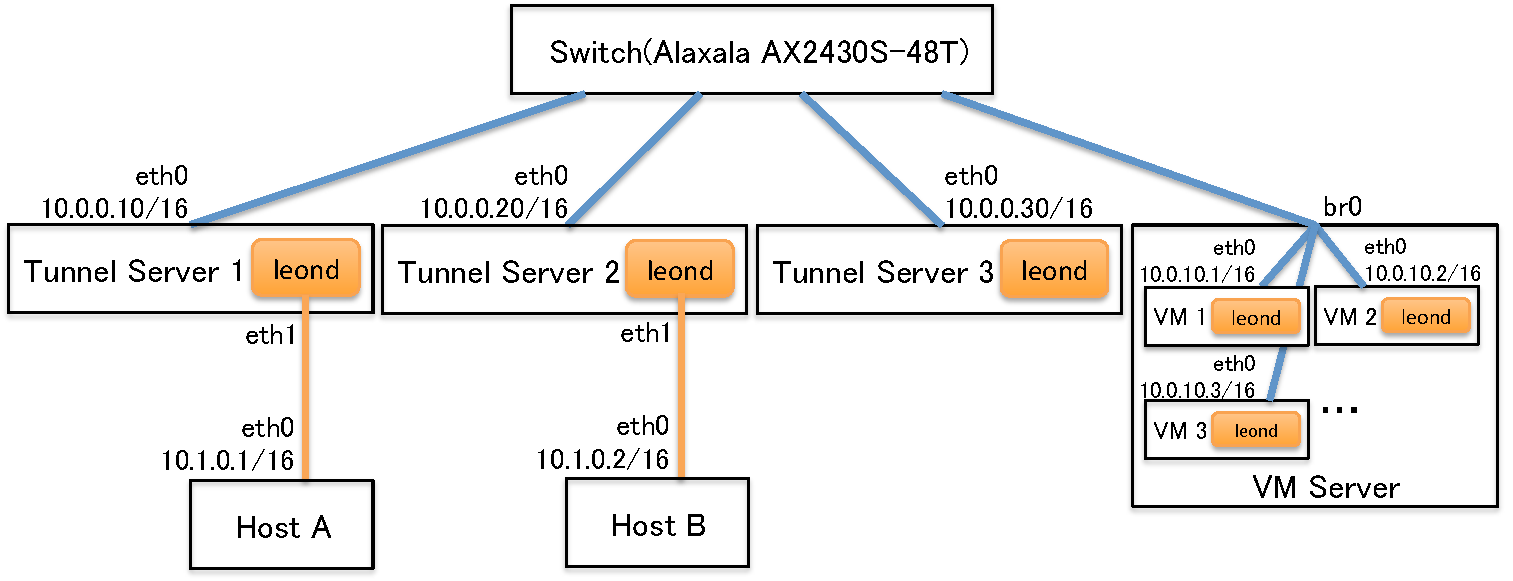
\includegraphics[scale=0.65]{./img/experimenttopology}
		\caption{実験環境のトポロジー図}
		\label{img:experimenttopology}
	\end{center}
\end{figure}

実験環境に対する要求から、本実験を行うにあたり、6台の実機サーバーを利用して実験環境を構築した。この実験環境のトポロジー図を図~\ref{img:experimenttopology}に示す。
また、利用した実機サーバーの仕様を表~\ref{table:expserv}に示す。更に、それぞれのサーバーで利用したソフトウェアのバージョンを
表~\ref{table:expversion}に示す。
6台の実機サーバーの内、3台でLEONの実装であるleondを動作させた。このうち2台に、実際に拡張されたLayer 2ネットワークに参加する
ホストサーバーとして実機サーバーを直接接続した。さらに、残りの実機サーバー1台で最大27台の仮想マシンを動作させ、仮想マシン内部で
leondを動作させた。leondが動作するサーバーは全て同じLayer 2ネットワークに所属している。

\begin{table}[h]
\begin{center}
	\caption{実験で利用した実機サーバーの仕様}
	\begin{tabular}{|l|l|l|l|}
		\hline
		ホスト & CPU & メモリー & NIC \\
		\hline
		\hline
		Tunnel Server 1 & Intel Xeon L5520 2.27Ghz & 12GB & NetXtreme II BCM5709 \\
		\hline
		Tunnel Server 2 & Intel Xeon L5520 2.27Ghz & 24GB & Intel 82575EB \\
		\hline
		Tunnel Server 3 & Intel Xeon E5430 2.66Ghz & 4GB & NetXtreme II BCM5708 \\
		\hline
		Host A & Intel Xeon 5160 3.00Ghz & 4GB & Intel 80003ES2LAN \\
		\hline
		Host B & Intel Xeon 5160 3.00Ghz & 4GB & Intel 80003ES2LAN \\
		\hline
		VM Server & AMD Opteron 6128 & 20GB & Intel 82576 \\
		\hline
	\end{tabular}
	\label{table:expserv}
\end{center}
\end{table}

\begin{table}[h]
\begin{center}
	\caption{実験で利用した各サーバーのバージョン}
	\begin{tabular}{|l|l|l|l|}
		\hline
		サーバー & OS & Linux Kernel & gcc \\
		\hline
		\hline
		Tunnel Server 1 & Debian GNU/Linux 6.0.6 Squeeze & 3.7.2 & 4.4.5 \\
		Tunnel Server 2 & 				 &       &       \\
		Tunnel Server 3	&				 &       &       \\
		VM \#		&				 & 	 &	 \\
		\hline
		Host A 		& Debian GNU/Linux 6.0.6 Squeeze & 2.6.32-5 & 4.4.5 \\
		Host B		&				 &	    &       \\
		\hline
		VM Server 	& Ubuntu 10.04.4 LTS		 & 3.7.2 & 4.4.3 \\
		\hline
	\end{tabular}
	\label{table:expversion}
\end{center}
\end{table}

また、leondが動作するサーバー間で、tc(Linux Traffic Control)~\cite{tc}を利用して擬似的に遅延を発生させた。サーバー間に設定した遅延を
図~\ref{img:experimenttc}に示す。全てのトンネル終端点において、Tunnel Server 3への遅延は他のサーバーへの遅延よりも小さく設定した。
これにより、直接通信するよりも小さい遅延で通信することができる経路を作成した。全てのサーバー間の通信は
Tunnel Server 3を経由することで、直接通信するよりも小さい遅延で通信をすることができる。仮想マシン間には遅延を設定していない。

\begin{figure}
	\begin{center}
		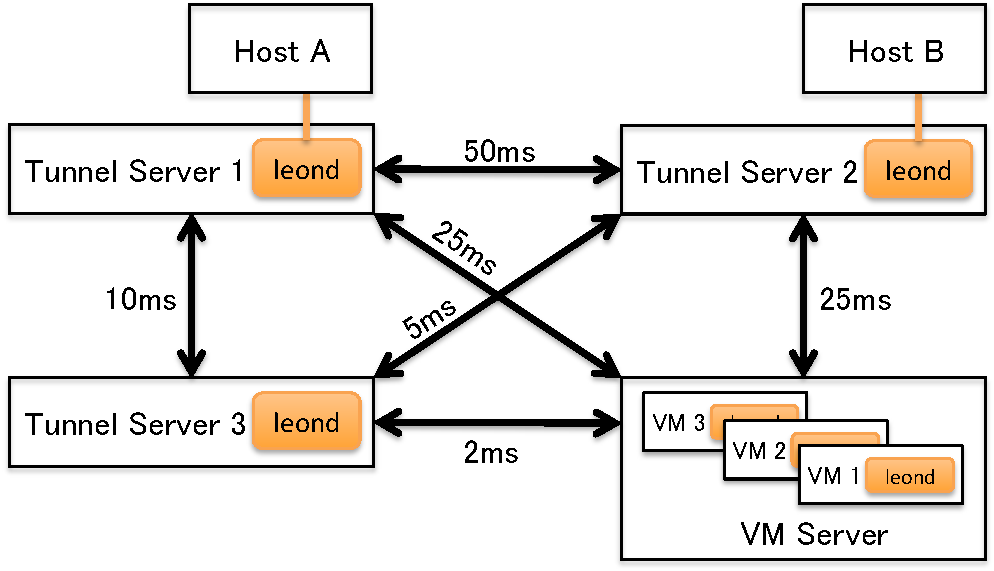
\includegraphics[scale=0.70]{./img/experimenttc}
		\caption{実験環境に設定された擬似的な遅延}
		\label{img:experimenttc}
	\end{center}
\end{figure}

これによって、実機サーバー6台を用いて、本実験を行うための要求を満たした実験環境を構築した。

\subsection{実験内容}
\label{experiment:spec}

本実験では、中継するトンネル終端点で障害が発生してから、全てのトンネル終端点でトポロジーが収束するまでの時間を計測する。
中継をするトンネル終端点で障害が発生すると、そのトンネル終端点を経由して行われていた通信は、トポロジーが収束するまで行えなくなる。
本実験では、この性質を利用してトポロジーの収束時間を計測するプログラムを作成した。本プログラムは、あるトンネル終端点から全てのトンネル終端点
に対して定期的にICMP Echo Requestを送信し、その返信を監視する。本プログラム開始後、中継を行なっているトンネル終端点
でネットワーク障害を発生させると、全てのトンネル終端点から返信がなくなる。返信がなくなると、中継するトンネル終端点で障害が発生したと判断し計測を開始する。
そして、全てのトンネル終端点でトポロジーが収束すると、全てのトンネル終端点から返信を受信できるようになる。本プログラムが全てのトンネル終端点から
返信を受け取ると、全てのトンネル終端点でトポロジーが収束したと判断し計測を終了する。

作成したプログラムはTunnel Server 1で動作させた。実験環境下でTunnel Server 1で動作するleondが構築する
Layer 2ネットワークのトポロジーと実験の様子を図~\ref{img:topologyat1}に示す。Tunnnel Server 1が、他のトンネル終端点へ
イーサネットフレームを転送する際には、必ずTunnel Server 3を経由する。作成したプログラムをTunnel Server 1で開始後、
Tunnel Server 3のネットワーク接続を切断した。Tunnel Server 3が切断されると、全てのトンネル終端点はTunnel Server 1と
通信ができなくなる。全てのトンネル終端点で動作するleondが、Tunnel Server 3での障害を検知すると、トポロジーが
再構築され、再びTunnel Server 1と通信ができるようになる。障害検知後のTunnel Server 1で動作するleondが構築する
トポロジーは図~\ref{img:topologyat1b}で示すようなトポロジーとなる。Tunnel Server 1と全てのトンネル終端点が
通信可能になった時点で計測終了である。

\begin{figure}
	\begin{center}
		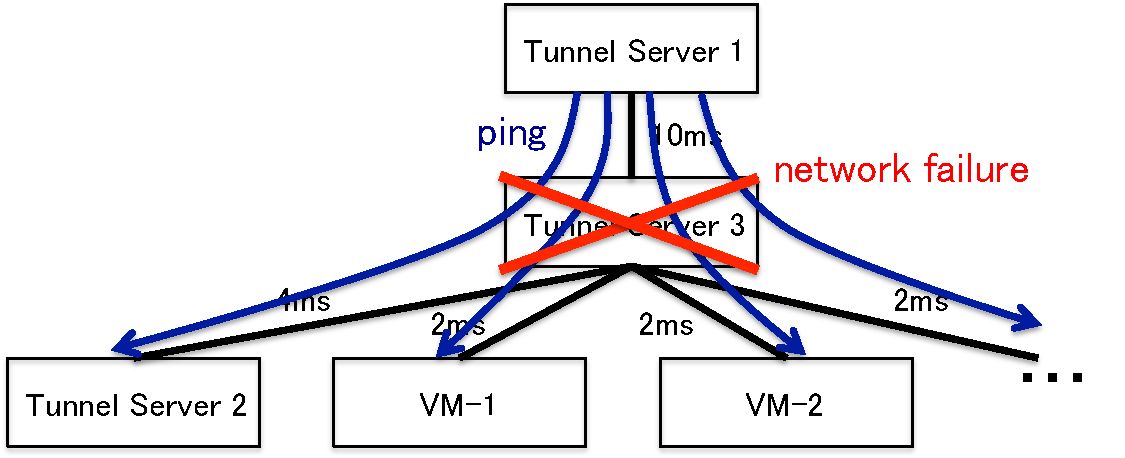
\includegraphics[scale=0.70]{./img/topologyat1}
		\caption{Tunnel Server 1で構築されるトポロジーと実験の様子}
		\label{img:topologyat1}
	\end{center}
\end{figure}

\begin{figure}
	\begin{center}
		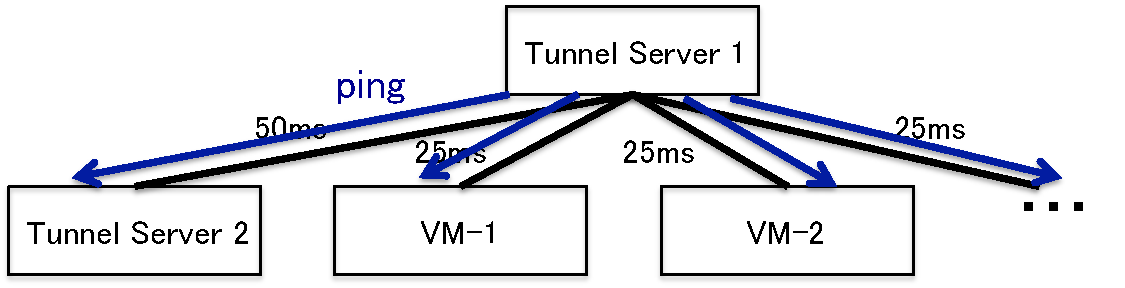
\includegraphics[scale=0.70]{./img/topologyat1b}
		\caption{トポロジー収束後のトポロジー}
		\label{img:topologyat1b}
	\end{center}
\end{figure}

\subsection{実験結果}
\label{experiment:result}

本実験では、3台から30台までのトンネル終端点を利用して拡張したLayer 2ネットワークにおいて、中継を行なっているトンネル終端点
での障害発生後、全てのトンネル終端点でトポロジーが収束するまでにかかった時間を計測した。その実験結果を図~\ref{graph:topology}に
示す。本実験では、3台から30台までの各トンネル終端点数について、~\ref{experiment:spec}節で説明した計測を5回行った。計測を
行う度に全てのトンネル終端点でleondを再起動し、Layer 2ネットワークの再構築を行った。

\begin{figure}
	\begin{center}
		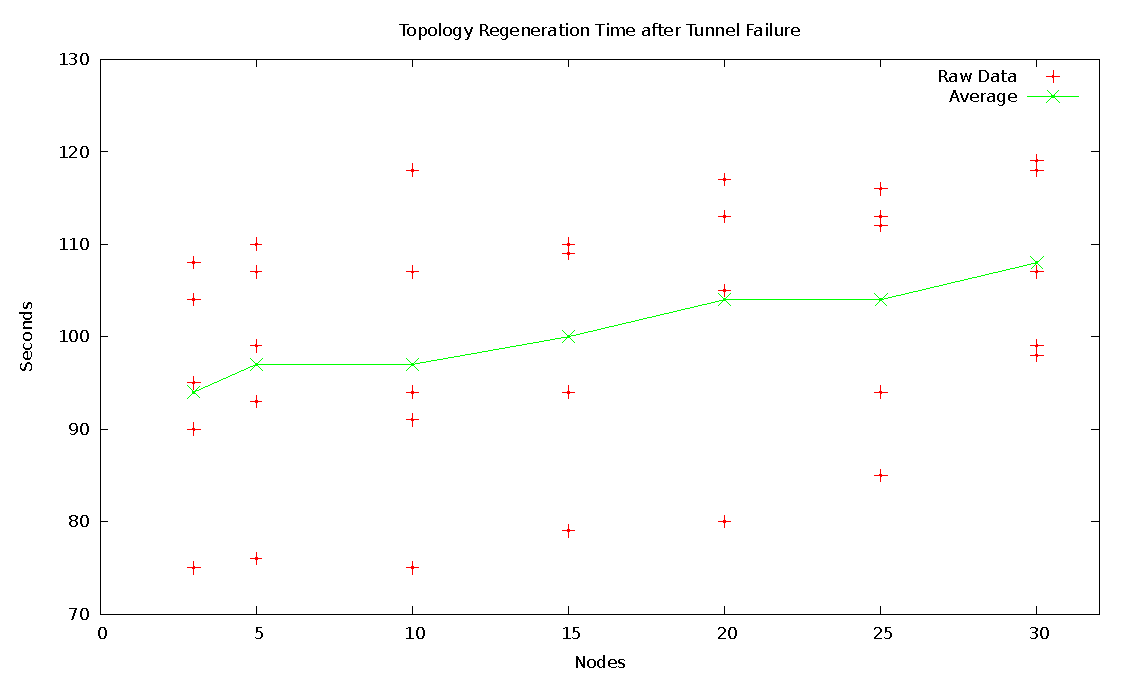
\includegraphics[scale=0.80]{./img/topology}
		\caption{ノード数に応じたトポロジー収束時間}
		\label{graph:topology}
	\end{center}
\end{figure}

図~\ref{graph:topology}から、中継を行なっているトンネル終端点で障害が発生してから全てのトンネル終端点でトポロジーが収束
するまでにかかる時間は、同じトンネル終端点の台数でもばらつきが大きいことがわかる。25台のトンネル終端点では、トポロジーの収束にかかった時間
は最小で81秒、最大で123秒と42秒の差がある。一方で、同じ台数でもばらつきはあるが、各台数の平均値から、台数が増加するに連れトポロジーが収束するまでに
かかる時間の平均値は緩やかに増加していることがわかる。そのため、Layer 2ネットワークに参加しているトンネル終端点の台数が増加するに連れ、
中継を行なっているトンネル終端点で障害が発生してから全てのトンネル終端点でトポロジーが収束するまでにかかる時間は少しずつ増加する、と考えられる。

\subsection{考察}

本研究では、トンネル終端点の増加による影響を評価した。そして本評価では、Layer 2ネットワークに参加しているトンネル終端点の台数が、中継を行なっているトンネル終端点において障害
が発生してから全てのトンネル終端点でトポロジーが収束するまでかかる時間に与える影響を調査した。調査をするにあたり、
擬似的に遅延を発生させ、直接通信するよりも小さい遅延で通信できる経路が存在する実験環境を構築し、評価実験を行った。
その結果、同じトンネル終端点の台数でも、トポロジーが収束する時間のばらつきは大きいが、各台数の平均値からトンネル終端点の
台数が増加するに連れ、トポロジーの収束にかかる時間は緩やかに増加する、ということがわかった。よって、トンネル終端点の増加は
LEONに悪影響を及ぼすということがわかった。

この原因は、トンネル終端点を起動した時間の差であると考えられる。あるトンネル終端点で、トンネル終端点の障害発生からトポロジー
の再構築までかかる時間を$ T $秒、遅延計測を行う間隔時間を$ T_p $秒、最後に遅延計測を行なってから障害発生までに経過した時間を$ T_e $秒
とすると、これらの関係を次の数式で表すことができる。

\begin{displaymath}
\displaystyle T = (T_p - T_e) + T_p
\end{displaymath}

遅延計測を行う間隔時間(=$ T_p $)はデフォルト状態で60秒である。LEONは遅延計測が2回失敗すると障害発生と判断するため、障害発生からトポロジー
の再構築までかかる時間(=$ T $)は、$ T_p $秒以上となる。例えば、最後に遅延計測を行なってから20秒経過した時点で障害が発生すると、それを検知し
トポロジーの再構築までかかる時間は$ T = (60 - 20) + 60 = 100 $より100秒である。障害発生からトポロジーの再構築までかかる時間(=$ T $)は、最後に遅延計測を
行なってから障害発生までに経過した時間(=$ T_e $)が小さいほど大きくなる。
トンネル終端点が複数の場合、全てのトンネル終端点を同時に起動をしていないので、$ T_e $の値にはトンネル終端点ごとにばらつきがある。
トンネル終端点の台数が増えると$ T_e $の値のばらつきが大きくなり、最後に遅延計測を行なってから障害発生までに経過した時間が短いトンネル終端点がいる確率が高まる。
そのため、トンネル終端点の台数が増加するに連れ、中継を行なっているトンネル終端点において障害が発生してから全てのトンネル終端点でトポロジーが収束するまでかかる時間
が増加すると考えられる。

RFC 793ではTCPのタイムアウト時間は300秒と定義されている~\cite{rfc:tcp}。第~\ref{rw}章で挙げたLayer 2ネットワーク拡張技術を利用して構築されたLayer 2ネットワークで障害が発生すると、
管理者が障害の原因を特定し、修正するまでに時間がかかる。この手法では、障害が発生してから修正まで300秒以上かかり、TCPのセッションが切断されてしまう場合が多い。LEONでは、
中継を行なっているトンネル終端点で障害が発生してから、最大120秒で通信が再び可能となる。そのため、LEONを用いることで、障害発生時はTCPのセッションが切断される前に復旧
することができる。

\section{実験のまとめ}

本研究では、インターネット上に分散した複数の拠点を用いて構築されたサービスのパフォーマンス改善を目標としている。従来手法では、複数拠点を用いて
サービスを構築した場合、サービスを構成するコンポーネントのパフォーマンスが遅延により低下してしまうため、サービスのパフォーマンスが低下してしまう
という問題があった。この問題を解決するため、LEONは遅延の最も小さい経路でイーサネットフレームの転送を行う。これにより、コンポーネントのパフォーマンス
が改善され、サービスのパフォーマンスが改善されるということがわかった。

しかし、一方でトンネル終端点の台数が増加するとLEONに悪影響を及ぼすということがわかった。トンネル終端点の増加が与える影響として、中継を行うトンネル終端
点で障害が発生してから、そのトンネル終端点を経由していた通信の復旧までにかかる時間の増加があるということもわかった。これはLEONが分散して動作するために、
Layer 2ネットワークに参加している全てのトンネル終端点が全てのトンネル終端点の管理、死活監視や遅延計測などを行う必要があるためであると考える。そのため、
LEONは多くの拠点に同一のLayer 2ネットワークを拡張するためには適していないということがわかった。

%%% Local Variables:
%%% mode: japanese-latex
%%% TeX-master: "../yummy_bthesis"
%%% End:

\chapter{結論}
\label{conclusion}

本章では、本論文のまとめと今後の展望を示す。

\section{本研究のまとめ}

本研究では、インターネット上の複数の拠点に同一のLayer 2ネットワークを拡張することができる一対多型のLayer 2ネットワーク
拡張技術であるLEONの設計と実装をした。現在のインターネットには、宛先と直接通信した場合より、他の拠点を経由して宛先と通信
した場合の方が、通信をする際の遅延が小さくなる場合がある。LEONはトンネル終端点間の遅延を計測し、その計測結果をもとに遅延が最も
遅延が小さくなる経路を計算する。これにより、LEONを利用することにより、イーサネットフレームを遅延の最も小さい経路で転送できるようになった。
その結果、本研究で行った実験から、LEONを利用して拡張されたLayer 2ネットワーク上で通信を行った場合、従来手法と比べ、
サービスを構成するコンポーネントのパフォーマンスが改善され、サービスのパフォーマンスも改善されるということがわかった。
しかし、LEONでは全てのトンネル終端点が他のトンネル終端点の状態管理や遅延計測などを行う必要があるため、
トンネル終端点が増加することによりトンネル終端点の負荷が高くなるため様々な悪影響が生じる。
本研究で行った実験から、トンネル終端点の増加が与える影響の1つとして、中継を行なっているトンネル終端点での障害発生から、そのトンネル終端点を経由していた通信が再び可能になるまで
かかる時間の増加があるということがわかった。そのため、LEONは多くの拠点にLayer 2ネットワークを拡張するには適していない
ということもわかった。

\section{今後の展望}

本研究で提案したLayer 2ネットワーク拡張技術であるLEONは、中継を行なっているトンネル終端点で障害が発生してから、
再びそのトンネル終端点を中継して行われていた通信が行えるようになるまで、最大で120秒かかる。そのため、最大120秒間、通信が行えない
間に、送信されたイーサネットフレームがパケットロスされてしまう可能性やサーバーから切断されてしまうなどといった
問題の原因となることが想定される。また、図~\ref{img:tenbou1}で示すように、ファイアーウォールの設定や拠点間のネットワーク
障害などにより、直接通信することはできないが、他のトンネル終端点からは到達することができる場合が考えられる。LEONは
このよう場合、直接通信することができないトンネル終端点は障害発生と判断し、トンネル終端点リストから消去してしまう。
そのため、Layer 2ネットワークが分断してしまうという問題がある。これらの問題を解決するためには、より優れた障害検知
の手法が必要である。

\begin{figure}
	\begin{center}
		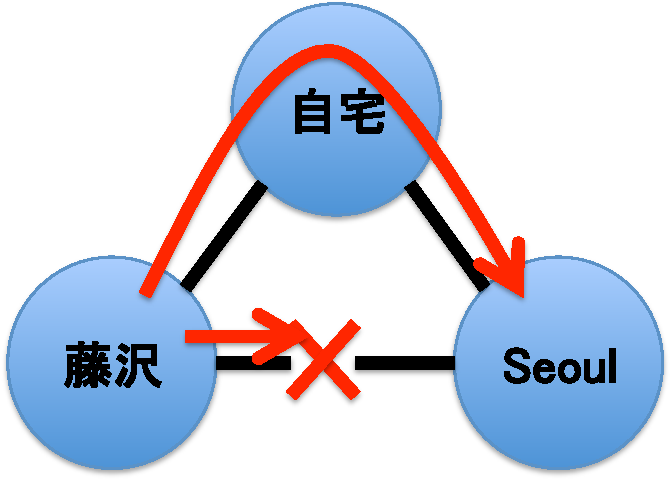
\includegraphics[scale=0.60]{./img/tenbou1}
		\caption{直接通信をすることができない状況}
		\label{img:tenbou1}
	\end{center}
\end{figure}

また、本研究で提案した手法は、トンネル終端点間の遅延を計測し、その計測結果をもとに経路の計算を行った。しかし、インターネット
には遅延は小さいが帯域幅は細いトンネル終端点や、遅延は大きいが帯域幅は太いトンネル終端点が存在する可能性がある。WIDE Cloudの
ように拡張されたLayer 2ネットワーク上で様々なアプリケーションが動作するような環境では、遅延よりも帯域幅を優先したほうがパフォーマンス
が高くなるアプリケーションも動作している可能性がある。そのため、Layer 2ネットワーク拡張技術はトンネル終端点間の遅延だけでなく、Layer 2ネットワーク上
で動作するアプリケーションやトンネル終端点間の帯域幅も考慮する必要がある。

%%% Local Variables:
%%% mode: japanese-latex
%%% TeX-master: "../yummy_bthesis"
%%% End:

\chapter*{謝辞}
\addcontentsline{toc}{chapter}{謝辞}
\label{thanks}

本論文の作成にあたり、ご指導いただきました慶應義塾大学環境情報学部教授村井純博士、同学部教授中村修博士、同学部准教授 Rodney D. Van Meter III 博士に感謝致します。

研究について日頃からご指導頂きました松谷健史氏、空閑洋平氏に感謝致します。
研究室に所属したばかりの頃から本研究に至るまで、特定の分野にこだわらない広い視点から絶えず多くのご指導をいただきました。
本研究を卒業論文としてまとめることができたのも両氏のおかげです。重ねて感謝申し上げます。

研究室を通じた生活の中で多くの示唆を与えてくださった髙橋俊成氏、Arch研究グループの皆様に感謝します。

また、徳田・村井・楠本・中村・高汐・バンミーター・植原・三次・中澤・武田合同研究プロジェクトの皆様に感謝致します。

%%% Local Variables:
%%% mode: japanese-latex
%%% TeX-master: "../yummy_bthesis"
%%% End:


\renewcommand{\thechapter}{\Alph{chapter}}
\setcounter{chapter}{0}
\vspace{-5mm}


\bibliographystyle{unsrt}\pagestyle{plain}
\bibliography{./bib/cites,./bib/bootstrapping_evidence,./bib/appendix}\pagestyle{plain}
\thispagestyle{empty}%bibtex


\end{document}

%%% Local Variables:
%%% mode: japanese-latex
%%% TeX-master: t
%%% End:
